%# -*- coding: utf-8-unix -*-
%%==================================================
\chapter{知识推理方法}\label{AIchap3}
%%%%%%%%%%%%%%%%%%%%%%%%%%%%%%%%%%%%
\begin{tcolorbox}[colback=white!50,colframe=orange!50,title=智能系统的推理过程]
\uwave{智能系统的推理过程实际上就是一种思维过程}. 按照推理过程所用知识的确定性, 推理可分为确定性推理和不确定性推理.
\end{tcolorbox}
%%%%%%%%%%%%%%%%%%%%%%%%%%%%%%%%%%%%%%%%%%
\begin{figure}[H]
\centering
\includegraphics[width=0.84\textwidth]{KRC412184.jpg}
\label{KRC412184004}
\end{figure}
%%%%%%%%%%%%%%%%%%%%%%%%%%%%%%%%%%

过去三十年,人们对知识的表示与推理(KRR)和机器学习(ML)领域地一些常见的问题进行了深入而广泛地探究, 如知识表示的类型、知识和数据的作用、信息的缺乏和过剩、解释和理解的需要 \cite{BouraouiKR2019}等问题.
%%%%%%%%%%%%%%%%%%%%%%%%%%%%%%%%%%%%%%%
\section{什么是推理}
%%%%%%%%%%%%%%%%%%%%%%%%%%%%%%%%%%%%%%%%%%
\begin{mydef}{推理}{1}
    是指按照某种策略, 从已知事实出发去推导出结论的过程.
\end{mydef}
%%%%%%%---------------------------------------------
\subsection{推理所用的事实}
\begin{itemize}
\item \textbf{初始证据}: 在推理前用户提供的详实佐证材料.
\item \textbf{中间结论}: 在推理过程中所得到的结果.
\item \textbf{推理过程}: 主要由推理机来完成, 所谓推理机就是智能系统中用来实现推理的程序.
\end{itemize}
%%%%%%%-----------------------------------------------
\begin{example}
  对于医疗专家系统, 专家知识保存在知识库中. 推理开始时, 先把病人的症状和检查结果放到综合数据库中, 然后再从综合数据库的初始证据出发, 按照某种策略在知识库中寻找, 并使用知识, 直到推出最终结论为止.
\end{example}

推理的两个基本问题(方法和策略):
\begin{itemize}
\item 推理的方法: 表达前提和结论的逻辑关系.
\item 推理的控制策略: 确定推理方向, 消解冲突策略.
\end{itemize}
%%%%%%%---------------------------------------------
\subsection{按推理的逻辑基础分类}
%%%%%%%---------------------------------------------
\paragraph{演绎推理}~{}
\begin{mydef}{演绎推理}{1}
演绎推理是从已有知识出发, 去推出蕴含在这些已知知识中的适合于某种个别情况的结论. 是一种由一般到个别的推理方法, 其核心是\textcolor[rgb]{0,0,1}{\textbf{三段论:假言推理、拒取式和假言三段论}}.
\end{mydef}

%%%%%%%------------------------------------------
\begin{example}
  假言三段论
$$A\rightarrow B, B\rightarrow C \Rightarrow A\rightarrow C.$$
\end{example}

常用的\uwave{三段论由三部分组成: 一个大前提、一个小前提和一个结论}. 其中, 大前提是已知的一般性知识或推理过程得到的判断; 小前提是关于某种具体情况或某个具体实例的判断.
\begin{remark}
    结论是由大前提推出的, 并且适合于小前提的判断.
\end{remark}

%%%%%%%------------------------------------------------
\begin{example}
有如下三个判断是一个三段论推理:

     \ding{172} 计算机系的学生都会编程序;   (一般性知识).

     \ding{173} 程强是计算机系的一位学生;   (具体情况).

     \ding{174} 程强会编程序.            (结论).
\end{example}
其中, \ding{172}是大前提; \ding{173}是小前提;\ding{174}是经演绎推出来的结论.
可见, 推出的结论是蕴含在大前提中, 是大前提的一个特例.
%%%%%%%---------------------------------------------
\subsubsection{归纳推理}
\vspace{0.3cm}
\begin{mydef}{归纳推理}{1}
    \textbf{归纳推理}是一种由个别到一般的推理方法.
\end{mydef}
\begin{example}
归纳推理的类型
\begin{itemize}
    \item 按照所选事例的广泛性可分为\uwave{完全归纳推理和不完全归纳推理}.
    \item 按照推理所使用的方法可分为\uwave{枚举、类比、统计和差异归纳推理}等.
\end{itemize}
\end{example}
%%%%%%%---------------------------------------------
\vspace{0.3cm}
\begin{mydef}{完全归纳推理}{1}
    是指在进行归纳时需要考察相应事物的全部对象, 并根据这些对象是否都具有某种属性, 推出该类事物是否具有此属性.
\end{mydef}
%%%%%%%---------------------------------------------
\vspace{0.3cm}
\begin{mydef}{不完全归纳推理}{1}
    指在进行归纳时只考察了事物的部分对象, 就得出了关于该事物的结论.
\end{mydef}
%%%%%%%---------------------------------------------
\vspace{0.3cm}
\begin{mydef}{枚举归纳推理}{1}
    指在进行归纳时, 如果已知某类事物中的有限个具体事物都具有某种属性, 则可推出该类事物都具有此种属性.
\end{mydef}
%%%%%%%------------------------------------------
\begin{example}
设有如下事例:

    王强是计算机系学生, 他会编程序;

    高华是计算机系学生, 她会编程序;

     ……                ……
%%%%%%%-----------------------------------------------
\end{example}
    当这些具体事例足够多时, 就可归纳出一个一般性的知识: \uwave{凡是计算机系的学生, 就一定会编程序}.
%%%%%%%---------------------------------------------
\vspace{0.3cm}
\begin{mydef}{类比归纳推理}{1}
指在两个或两类事物有许多属性都相同或相似的基础上, 推理出它们在其他属性上也相同或相似的一种归纳推理方法.
\end{mydef}
设$A$、$B$分别是两类事物的集合:
\begin{align*}
  A&=\{a_1,a_2,\cdots\},\\
  B&=\{b_1,b_2,\cdots\}.
\end{align*}
并设$a_i$与$b_i$总是成对出现, 且当$a_i$有属性$P$时, $b_i$就有属性$Q$与此对应, 即
\begin{align*}
  P(a_i)\rightarrow Q(b_i),\,i=1,2,\cdots.
\end{align*}
     则当$A$与$B$中有一新的元素对出现时, 若已知$a'$有属性$P$, $b'$有属性$Q$, 即
\begin{align*}
  P(a')\rightarrow Q(b').
\end{align*}
%%%%------------------------------------------------------
\begin{example}
  使用SARS的相关经验去处理武汉发生的新型冠状病毒肺炎.
\end{example}
%%%%------------------------------------------------------
\begin{remark}
类比归纳推理的基础是相似原理, 其可靠程度取决于两个或两类事物的相似程度,或者这两类事物的相同属性与新属性之间的相关程度.
\end{remark}
%%%%%%%---------------------------------------------
\subsubsection{演绎推理与归纳推理的区别}
演绎推理是在已知领域内的一般性知识的前提下, 通过演绎求解一个具体问题或者证明一个结论的正确性. 它所得出的结论实际上早已蕴含在一般性知识的前提中, 演绎推理只不过是将已有事实揭露出来, 因此它不能增殖新知识.

归纳推理所推出的结论是没有包含在前提内容中的. 这种由个别事物或现象推出一般性知识的过程, 是增殖新知识的过程.

演绎推理是一种以严格的经典逻辑为基础的推理(MIT, Winston教授), 而不确定性推理本质上是一种非演绎推理, 虽然演绎推理也是一种人类的智能活动, 而人工智能中的推理主要是指\textbf{不确定性逻辑推理}, 也称之为\textbf{常识推理}.
\begin{itemize}
\item 演绎推理使用的是抽象而严格的定义, 它在一定理论框架下是绝对正确的定理和公式. 而常识推理使用的是具有局部与暂时合理性的知识和超知识, 即人们的共识和个人的经验.
\item 演绎推理有一定抽象的理论承诺, 它所使用的概念是清晰的, 任何时候都有相同的含义, 因而是确定的. 而常识推理使用的概念是模糊的, 不确定的, 对于不同的人可能会有不同的理解, 具有不确定性, 而知识中的不肯定性表现了人类认识的局限性, 普遍知识中可能有一部分具体对象不正确, 超知识的不肯定性表现在个人的主观性, 特殊知识较之全面知识, 具有片面性.
\item 演绎推理是一种“保真”的推理, 也就是前提正确, 那么由前提经演绎推出的结论也正确, 而常识推理是一种“未必保真”的推理, 即使前提正确, 其结论也未必正确, 是一种近似保真而具有直观合理性的结论.
\item 演绎推理是具有相容性的推理, 在一个理论体系中不可能推出两个同时成立且相反的命题, 而常识推理具有矛盾性, 是一种非协调推理, 在一个知识系统中可能会得到两个相反的结论.
\item 演绎推理是完全的, 具有单调性, 增加新的事例不会影响原有的结论, 而常识推理是不完全的非单调性推理, 增加新的事例可能会影响原有的结论.
\end{itemize}

总体来说, 演绎推理是在抽象的逻辑结构上进行的, 是一种从普遍性到特殊性的推理,

1) 它不承认任何由已知前提推不出的结论,

2) 不承认任何不经过演绎推理的假设,

3) 不承认任何含有例外事例的结论。

演绎推理是一种让人“放心”, 而偏于”保守“的推理机制. 而常识推理是在实践和经验的基础上进行的, 是一种从特殊性到普遍性的推理, 具有“容错”的特征.
通过不断的发现矛盾与限制矛盾, 修正和维护知识, 其知识的正确性, 既不取决于逻辑的推理规则, 也不取决于以知识为前提的推理过程, 而是取决于推理的结果与事实的符合程度.

演绎推理的真值只能是或“真”或“假”.
常识推理的真值可以是从“真”到“假”之间的任意一个过渡值. 因此, 在常识推理中, 往往会用一种确定度来表示结果的真实程度.
而在正畸思维中, 往往是这样一种常识推理的心理思维活动在其中起决定性作用, 因此, 如何将常识推理, 或说不确定性推理的思维活动采用定量的形式让计算机处理, 将会大大提高数字化人工智能正畸技术的发展.
%%%%%%%---------------------------------------------
\begin{example}
  一位计算机维修员, 从书本知识开始学习, 到通过大量实例积累起来丰富的经验这一过程就 是一种归纳推理方式. 运用这些一般性知识去维修计算机的过程则是演绎推理.
\end{example}
%%%%%%%---------------------------------------------
\subsection{推理的控制策略及分类}
%%%%%%%---------------------------------------------
\subsubsection{推理的控制策略}
\begin{itemize}
\item 推理过程不仅依赖于所用的推理方法, 同时也依赖于推理的控制策略.
\item 推理的控制策略是指给出使用领域知识的方式, 使推理过程尽快达到目标的策略.
\end{itemize}
%%%%%%%---------------------------------------------
\paragraph{控制策略的分类}~{}
由于智能系统的推理过程一般表现为一种搜索过程, 因此, 推理的控制策略又可分为\uwave{推理策略}和\uwave{搜索策略}.
\begin{itemize}
\item 推理策略: 主要解决推理方向和推理冲突等问题, 如推理方向控制策略、求解策略、限制策略和冲突消解策略等.
    \begin{itemize}
    \item 推理方向控制策略用于确定推理的方向控制, 可分为正向推理、逆向推理、混合推理及双向推理.
    \item 求解策略是指仅求一个解, 还是求所有解或最优解等.
    \item 限制策略是指对推理的深度、宽度、时间和空间等进行的限制.
    \item 冲突消解策略是指当推理过程有多条知识可用时, 如何从这多条可用知识中选出一条最佳知识用于推理的策略.
    \end{itemize}
\item 搜索策略: 主要解决推理线路、推理效果和推理效率等问题.
\end{itemize}
本章主要讨论推理策略, 至于搜索策略将放到第\ref{AIchap4}章单独讨论.
%%%%%%%---------------------------------------------
\subsection{正向推理}
\begin{mydef}{前向链推理}{1}
从已知事实出发、正向使用推理规则, 亦称为\uwave{数据驱动推理或前向链推理}.
\end{mydef}
\subsubsection{正向推理的算法描述}

(1) 把用户提供的初始证据放入综合数据库;

(2) 检查综合数据库中是否包含了问题的解, 若已包含, 则求解结束, 并成功退出;否则执行下一步;

(3) 检查知识库中是否有可用知识, 若有, 形成当前可用知识集, 执行下一步;否则转(5).

(4) 按照某种冲突消解策略, 从当前可用知识集中选出一条规则进行推理, 并将推出的新事实加入综合数据库中, 然后转(2).

(5) 询问用户是否可以进一步补充新的事实, 若可补充, 则将补充的新事实加入综合数据库中, 然后转(3); 否则表示无解, 失败退出.

至于如何根据综合数据库中的事实到知识库中选取可用知识, 当知识库中有多条知识可用时, 应先使用哪一条知识等. 这些问题涉及到了知识的匹配方法和冲突消解策略, 以后将会分别讨论.
正向推理求解的算法流程如图\ref{AI32fig12}所示:
%%%%%%%-----------------------------------------------%
%\begin{figure}[H]
%\centering
%\includegraphics[width=0.6\textwidth]{zhengxiangtuili2019112512.PNG}
%\caption{正向推理的算法流程}
%\label{AI32fig12}
%\end{figure}
%%%%%%%%%%%%%%%%%%%%%%%%%%%%%%
\begin{figure}[H]
\begin{center}
    \begin{tikzpicture}[decision/.style={diamond, draw, fill=blue!20, text width=3.5cm, aspect=5,align=flush center, inner sep=0pt},font={\sf \small},scale=0.78]
        \def \smbwd{2cm}
        \def \smbwe{4cm}
        %定义流程图的具体形状
        \node (InitDB) at (0,-0.75) [draw, process,minimum width=\smbwd, minimum height=0.5cm] {把初始证据放入DB};               % 把初始证据放入DB
        \node (IsDBsolvable)[draw,decision,align=center,below=0.5cm of InitDB,minimum width=\smbwd] {DB中有解吗?};              %DB中有解吗?
        \node (leftabove0)[yshift=0.7cm,left=0.6cm of IsDBsolvable] {};
        \node (IsKNavailable)[draw,decision,align=center,below=0.5cm of IsDBsolvable] {KB中有可用知识吗?};                       %KB中有可用知识吗
        \node (KNset)[draw, process,align=center,below=0.5cm of IsKNavailable] {形成可用知识集};                                 %形成可用知识
        \node (IsKNsetEmpty)[draw,decision,align=center,below=0.5cm of KNset,minimum width=\smbwd] {可用知识集空?};              %可用知识集空
        \node (leftabove1)[yshift=0.7cm,left=0.2cm of IsKNsetEmpty] {};
        \node (CollapSolve)[draw, process,align=center,below=0.5cm of IsKNsetEmpty] {执行冲突消解策略};                          %冲突消解
        \node (IsNewKN)[draw,decision,align=center,below=0.5cm of CollapSolve,minimum width=\smbwd] {是新知识吗?};              %是新知识吗
        \node (AddtoKB)[draw, process,align=center,below=0.5cm of IsNewKN] {将新事实加入到DB};                                   %将新事实加入到DB

        \draw[->] (InitDB)--(IsDBsolvable);
        \draw[->] (IsDBsolvable)node[left,yshift=-0.7cm] {$N$}--(IsKNavailable);
        \draw[->] (IsKNavailable)node[left,yshift=-0.7cm] {$Y$}--(KNset);
        \draw[->] (KNset)--(IsKNsetEmpty);
        \draw[->] (IsKNsetEmpty)node[left,yshift=-0.7cm] {$N$}--(CollapSolve);
        \draw[->] (CollapSolve)--(IsNewKN);
        \draw[->] (IsNewKN)node[left,yshift=-0.7cm,xshift=-.10cm]{$Y$}--(AddtoKB);
        \draw[->] (IsNewKN)node[left,xshift=-2.53cm,yshift=0.1cm]{$N$}-|(leftabove1.center)-|(IsKNsetEmpty.north);
        \draw[->] (AddtoKB)-|(leftabove0.center)-|(IsDBsolvable.north);

        \node (AddNewFact)[draw,decision,align=center,right=0.8cm of IsKNsetEmpty] {可补充新事实吗?};                             %可补充新事实吗
        \node (FailQuit)[draw, process,align=center,below=0.8cm of AddNewFact] {失败退出};                                       %失败退出
        \draw[->] (AddNewFact)node[left,yshift=-0.8cm] {$N$}--(FailQuit);
        \draw[->] (IsKNsetEmpty)node[left,xshift=3.34cm,yshift=-0.25cm]{$Y$}--(AddNewFact);
        \draw[->] (IsKNavailable.east)node[left,xshift=0.9cm,yshift=-0.3cm]{$N$}-|(AddNewFact.north);

        \node (SuccQuit)[draw,process,align=center,right=1.5cm of IsDBsolvable] {成功退出};
        \draw[->] (IsDBsolvable)node[left,xshift=3.18cm, yshift=-0.2cm]{$Y$}--(SuccQuit);

        \node (AddNewtop)[draw,process,align=center,xshift=2.3cm,below=-0.1cm of SuccQuit] {把补充的事\\实加入DB};
        \draw[->] (AddNewFact.east)|-node[left,xshift=0.1cm, yshift=-0.2cm]{$Y$}(AddNewtop.east);
        \draw[->] (AddNewtop)-|(IsKNavailable.north);
     \end{tikzpicture}
    \vspace{-0.2cm}
    \caption{正向推理求解的算法流程}
    \label{AI32fig12}
\end{center}
\end{figure}
%%%%%%%-----------------------------------------------
\begin{example}
请用正向推理完成以下问题的求解. 假设知识库中包含有以下2条规则:
\begin{align*}
            &r_1: \,\,   \textup{IF}\,\,     B\,\,     \textup{THEN}\,\,     C;\\
            &r_2: \,\,   \textup{IF}\,\,     A\,\,     \textup{THEN}\,\,     B.
\end{align*}
已知初始证据$A$, 求证目标$C$.
\end{example}
%%%%%%%----------------------------------------%%
\begin{result}
本例的推理过程如下:
\begin{itemize}
\item 推理开始前, 综合数据库为空.
\item 推理开始后, 先把$A$放入综合数据库, 然后检查综合数据库中是否含有该问题的解, 回答为“$N$”.
\item 接着检查知识库中是否有可用知识, 显然$r_2$可用, 形成仅含$r_2$的知识集. 从该知识集中取出$r_2$, 推出新的实事$B$, 将$B$加入综合数据库, 检查综合数据库中是否含有目标$C$, 回答为“$N$”.
\item 再检查知识库中是否有可用知识, 此时由于$B$的加入使得$r_1$为可用, 形成仅含$r_1$的知识集. 从该知识集中取出$r_1$, 推出新的实事$C$, 将$C$加入综合数据库, 检查综合数据库中是否含有目标$C$, 回答为“$Y$”.

它说明综合数据库中已经含有问题的解, 推理成功结束, 目标$C$得证.
\end{itemize}
\end{result}
%%%%%%%---------------------------------------------
\paragraph{正向推理的主要优点}
推理过程比较直观, 用户可以主动提供有用的事实信息, 适合于诊断、设计、预测和监控等领域的问题求解.
%%%%%%%---------------------------------------------
\paragraph{正向推理的主要缺点}
推理无明确目标, 求解问题时可能会执行许多与解无关的操作, 导致推理效率较低.
%%%%%%%---------------------------------------------
\subsubsection{逆向推理}

从某个假设目标出发, 逆向使用规则, 亦称为\textbf{目标驱动推理}或\textbf{逆向链推理}.
其算法流程如图\ref{AI32fig13}:
%%%%%%%-----------------------------------------------
%\begin{figure}[H]
%\centering
%\includegraphics[width=0.6\textwidth]{zhengxiangtuili2019112513.PNG}
%\caption{逆向链推理的流程图}
%\label{AI32fig13}
%\end{figure}
%%%%%%%-----------------------------------------------
\subparagraph{算法描述}~{}

(1) 将要求证的目标(假设)构成一个假设集;

(2) 从假设集中选出一个假设, 检查该假设是否存在于综合数据库中, 若在, 则该假设成立, 若此时假设集为空, 则成功退出, 否则仍执行(2); 若该假设不在数据库中, 则执行下一步;

(3) 检查该假设是否可由知识库的某个知识导出, 若不能由某个知识导出, 则询问用户该假设是否是可由用户证实的原始事实, 若是, 该假设成立, 并将其放入综合数据库, 再重新寻找新的假设, 若不是, 则转(5); 若能由某个知识导出, 则执行下一步;

(4) 将知识库中可以导出该假设的所有知识构成一个可用知识集;

(5) 检查可用知识集是否为空, 若是, 失败退出; 否则执行下一步;

(6) 按冲突消解策略从可用知识集中取出一个知识, 继续执行下一步;

(7) 将知识前提中的每个子条件都作为新的假设放入假设集, 然后转(2).

\begin{figure}[H]
\begin{center}
    \begin{tikzpicture}[decision/.style={diamond, draw, fill=blue!20, text width=5.5cm, aspect=5,align=flush center, inner sep=0pt},font={\sf \small},scale=0.5]
        \def \smbwd{2cm}
        \def \smbwe{4cm}
        %定义流程图的具体形状
        \node (InitDB) at (0,-0.75) [draw, process,minimum width=\smbwd, minimum height=0.5cm] {初始化DB和假设};                            % 初始化DB和假设
        \node (IsDBsolvable)[draw,process,align=center,below=0.5cm of InitDB,minimum width=\smbwd] {取出一个假设};                          %取出一个假设
        \node (leftabove0)[yshift=0.5cm,left=2.5cm of IsDBsolvable] {};
        \node (IsKNavailable)[draw,decision,align=center,below=0.5cm of IsDBsolvable] {假设是DB中的事实吗?};                                  %假设是B中的事实吗
        \node (KNset)[draw, decision,align=center,below=1.5cm of IsKNavailable] {假设能被KB中的知识导出吗?};                                  %假设能被KB中的知识导出吗
        \node (IsKNsetEmpty)[draw, process,align=center,below=0.5cm of KNset,minimum width=\smbwd] {将KB中所有能导出此假设\\的知识组成可用知识集}; %将KB中所有能导出此假设的知识组成可用知识集
        \node (CollapSolve)[draw, decision,align=center,below=0.5cm of IsKNsetEmpty] {可用知识集空吗?};                                      %冲突消解
        \node (IsNewKN)[draw, process,align=center,below=0.5cm of CollapSolve,minimum width=\smbwd] {利用冲突消解策略, 选取一条知识};           %利用冲突消解策略, 选取一条知识
        \node (AddtoKB)[draw, process,align=center,below=0.5cm of IsNewKN] {将知识前提中的子条件加入假设集};                                    %将知识前提中的子条件加入假设集

        \draw[->] (InitDB)--(IsDBsolvable);
        \draw[->] (IsDBsolvable)--(IsKNavailable);
        \draw[->] (IsKNavailable)node[left,yshift=-0.9cm] {$N$}--(KNset);
        \draw[->] (KNset)node[left,yshift=-0.9cm] {$Y$}--(IsKNsetEmpty);
        \draw[->] (IsKNsetEmpty)--(CollapSolve);
        \draw[->] (CollapSolve)node[left,yshift=-0.9cm] {$N$}--(IsNewKN);
        \draw[->] (IsNewKN)--(AddtoKB);
        \draw[->] (AddtoKB)-|(leftabove0.center)-|(IsDBsolvable.north);

        \node (QueryNewFact)[draw,diamond, fill=blue!20, aspect=1,text width=1.5cm, align=center,right=0.8cm of KNset] {询问用户\\有此\\事实吗?};                                          %可补充新事实吗
        \node (ToDB)[draw, process,align=center,right=0.6cm of QueryNewFact]{假设\\成立\\并放\\入DB};
        \draw[->] (QueryNewFact)--(ToDB);
        \draw[->] (KNset)node[left,xshift=4.4cm,yshift=-0.2cm] {$N$}--(QueryNewFact);
        \draw[->] (QueryNewFact)node[left,yshift=-1.8cm]{$N$}|-(CollapSolve.north);
        \node (FailQuit)[draw, process,align=center,right=1.3cm of CollapSolve]{失败退出};                                                  %失败退出
        \draw[->] (CollapSolve)node[left,xshift=4.2cm,yshift=-0.2cm] {$Y$}--(FailQuit);
        \node (AddNewtop)[draw,process,align=center,xshift=1.8cm,right=0.6cm of IsKNavailable] {该假设成立};
        \draw[->] (IsKNavailable)node[left,xshift=4.6cm,yshift=-0.2cm] {$Y$}--(AddNewtop);

        \node (NewAssu)[draw,process,align=center,right=1.3cm of AddNewtop] {还有\\新的\\假设吗?};
        \node (SuccQuit)[draw,process,align=center,below=5cm of NewAssu] {成功退出};
        \draw[->] (AddNewtop)--(NewAssu);
        \draw[->] (NewAssu)node[left,yshift=-1.35cm] {$N$}--(SuccQuit);
        \draw[->] (ToDB)|-(NewAssu);
        \draw[->] (NewAssu)|-(IsDBsolvable.east);
    \end{tikzpicture}
    \vspace{-0.2cm}
    \caption{逆向链推理的流程图}
    \label{AI32fig13}
\end{center}
\end{figure}
%%%%%%%-----------------------------------------------
对上例, 采用逆向推理, 其推理过程如下:
\begin{itemize}
\item 推理开始前, 综合数据库和假设集均为空.
\item 推理开始后, 先将初始证据$A$放入综合数据库, 目标$C$放入假设集, 然后从假设集中取出一个假设$C$, 查找$C$是否为综合数据库中的已知事实, 回答为“$N$”.
\item 再检查$C$是否能被知识库中的知识所导出, 发现$C$可由$r_1$导出, 于是$r_1$被放入可用知识集. 由于知识库中只有$r_1$可用, 故可用知识集中仅含$r_1$.
\item 接着从可用知识集中取出$r_1$, 将其前提条件$B$作为新的假设放入假设集. 从假设集中取出$B$, 检查$B$是否为综合数据库中的事实, 回答为“$N$”. 再检查$B$是否能被知识库中的知识所导出, 发现$B$可由$r_2$导出, 于是$r_2$被放入可用知识集. 由于知识库中只有$r_2$可用, 故可用知识集中仅含$r_2$.
\item 从可用知识集中取出$r_2$, 将其前提条件$A$作为新的假设放入假设集. 然后从假设集中取出$A$, 检查$A$是否为综合数据库中的事实, 回答为“$Y$”.

    说明该假设成立, 由于无新的假设, 故推理过程成功结束, 于是目标$C$得证.
\end{itemize}
%%%%%%%----------------------------------------%%
\paragraph{优缺点}
\begin{itemize}
\item 逆向推理的主要优点:
\begin{itemize}
\item 不必寻找和使用那些与假设目标无关的信息和知识;
\item 推理过程的目标明确;
\item 也有利于向用户提供解释, 在诊断性专家系统中较为有效.
\end{itemize}
\end{itemize}

\begin{itemize}
\item 逆向推理的主要缺点:
\begin{itemize}
\item 当用户对推理过程认识不清楚时, 由系统自主选择假设目标, 盲目性比较大, 若选择不好, 可能需要多次提出假设, 会影响系统效率.
\end{itemize}
\end{itemize}
%%%%%%%---------------------------------------------
\subsection{混合推理的概念}
把正向推理和逆向推理结合起来所进行的推理称为混合推理. 是一种解决较复杂问题的方法.
%%%%%%%---------------------------------------------
\subsubsection{混合推理的方法}
\begin{itemize}
\item \textbf{先正向后逆向}: 这种方法先进行正向推理, 从已知事实出发推出部分结果, 然后再用逆向推理对这些结果进行证实或提高它们的可信度.
\item \textbf{先逆向后正向}: 这种方法先进行逆向推理, 从假设目标出发推出一些中间假设, 然后再用正向推理对这些中间假设进行证实.
\item \textbf{双向混合}:是指正向推理和逆向推理同时进行, 使推理过程在中间的某一步结合起来. 对于这些方法不再详细讨论.
\end{itemize}
%%%%%%%---------------------------------------------
\section{逻辑学与人工智能}

人工智能的产生和发展与逻辑学密不可分. 逻辑学为人工智能的研究提供了根本观点与方法, 而逻辑方法则是人工智能研究中的主要工具. 本节从逻辑学为人工智能的研究提供理论基础出发, 讨论经典逻辑和非经典逻辑在人工智能中的应用, 以及人工智能在逻辑学发展方向上的影响.

人工智能主要研究用计算机方法模拟和扩展人的智能, 最终实现机器智能. 人工智能的研究与人的思维研究密切相关. 逻辑学始终是人工智能研究中的基础科学问题, 它为人工智能研究提供了根本方法.

%%%%%%%---------------------------------------------
\subsection{人工智能学科的诞生}
\subsubsection{经典数理逻辑的主要理论成果}
1) 西班牙的罗门$\cdot$卢乐(12世纪末13世纪初)提出制造可解决各种问题的通用逻辑机.

2) 17世纪, 英国的弗朗西斯·培根(Francis Bacon, 1561-1626年)在《新工具》中提出了归纳法. 随后, 德国莱布尼兹做出了四则运算的手摇计算器, 并提出了“通用符号”和“推理计算”的思想.

3) 19世纪, 英国乔治·布尔(George Boole, 1815-1864)创立了布尔代数, 奠定了现代形式逻辑研究的基础. 德国弗里德里希·路德维希·戈特洛布·弗雷格(德语:Friedrich Ludwig Gottlob Frege; 1848年11月8日—1925年7月26日)完善了命题逻辑, 创建了一阶谓词演算系统.

4) 20世纪初, 哥德尔对一阶谓词完全性定理与$N$形式系统的不完全性定理进行了证明. 在此基础上, 克林对一般递归函数理论作了深入的研究, 建立了演算理论. 英国艾伦·麦席森·图灵(Alan Mathison Turing, 1912年6月23日—1954年6月7日)建立了描述算法的机械性思维过程, 提出了理想计算机模型(即图灵机), 创立了自动机理论.

5) 1945年匈牙利冯$\cdot$诺依曼提出存储程序的思想和建立通用电子数字计算机的冯$\cdot$诺依曼型体系结构, 此外, 1946年, 美国的莫克利和埃克特成功研制出世界上第一台通用电子数学计算机ENIAC做出了开拓性的贡献.
%%%%-----------------------------------
\begin{remark}
经典数理逻辑的理论成果为1956年人工智能学科的诞生奠定了坚实的逻辑基础.

现代逻辑发展动力主要来自于数学中的公理化运动. 20世纪逻辑研究严重数学化, 发展出来的逻辑被恰当地称为“数理逻辑”, 它增强了逻辑研究的深度, 使逻辑学的发展继古希腊逻辑、欧洲中世纪逻辑之后进入第三个高峰期, 并且对整个现代科学产生了非常重要的影响.
\end{remark}

%%%%%%%---------------------------------------------
\subsection{逻辑学的发展}
%%%%%%%---------------------------------------------
\subsubsection{逻辑学的分类}

逻辑学是一门研究\uwave{思维形式及思维规律}的科学.  从17世纪德国数学家和哲学家莱布尼兹(G. Leibniz)提出数理逻辑以来, 随着人工智能的一步步的发展, 各种各样的逻辑也随之产生.
逻辑学大体上可分为\uwave{经典逻辑、非经典逻辑和现代逻辑}.

1) 经典逻辑与模态逻辑都是二值逻辑.

2) 多值逻辑是具有多个命题真值的逻辑, 是向模糊逻辑的逼近.

3) 模糊逻辑是处理具有模糊性命题的逻辑.

4) 概率逻辑是研究基于逻辑的概率推理.
%%%%%%%---------------------------------------------
\subsubsection{泛逻辑的基本原理}

当今人工智能深入发展遇到的一个重大难题就是专家经验知识和常识的推理. 迫切需要有一个可靠的逻辑, 不精确推理的逻辑学可以作为它们进一步研究信息不完全情况下推理的基础理论, 进而形成一种能包容一切逻辑形态和推理模式, 灵活开放自适应的逻辑学, 这便是柔性逻辑学. 而泛逻辑学就是研究刚性逻辑学(数理逻辑)和柔性逻辑学共同规律的逻辑学.

泛逻辑是从更高层面来研究所有形式逻辑的一般规律, 希望建立一种能包容一切逻辑形态和推理模式, 并能根据需要自由伸缩变化的柔性逻辑学, 刚性逻辑学将作为一个最小的内核存在其中, 这就是提出泛逻辑的根本原因, 也是泛逻辑的最终历史使命.
%%%%%%%---------------------------------------------
\subsection{逻辑学在人工智能学科的研究方面的应用}

逻辑方法是人工智能研究中的主要工具, 逻辑学的研究成果不但为人工智能学科的诞生奠定了理论基础, 而且它们还作为重要的成分被应用于人工智能系统中.
%%%%%%%---------------------------------------------
\subsubsection{经典逻辑的应用}

人工智能诞生后的20年间是逻辑推理占统治地位的时期. 1963年, 纽厄尔、西蒙等人编制的“逻辑理论机”数学定理证明程序(LT). 在此基础之上, 纽厄尔和西蒙编制了通用问题求解程序(GPS), 开拓了人工智能“问题求解”的一大领域. 经典数理逻辑只是数学化的形式逻辑, 只能满足人工智能的部分需要.
%%%%%%%---------------------------------------------
\subsubsection{非经典逻辑的应用}

(1) \textbf{不确定性的推理研究}

人工智能是用\uwave{数值的方法表示和处理不确定信息的方法}, 即给系统中每个语句或公式赋一个数值, 用来表示语句的不确定或确定性. 比较具有代表性的单个模型有: 1976年杜达提出的主观贝叶斯模型, 1978年扎德提出的可能性模型, 1984年邦迪提出的发生率计算模型, 以及假设推理、定性推理和证据空间理论等经验性模型.

在人工智能中, 可把归纳看成是从个别到一般的推理. \uwave{归纳逻辑是关于或然性推理的逻辑}.
借助这种归纳方法和运用类比的方法, 计算机就可以通过问题的相似性, 从相应的知识库中调用有关知识来处理新问题.

(2) \textbf{不完全信息的推理研究}

常识推理是一种非单调逻辑推理方法, 即人们基于不完全的信息推出某些结论, 当人们得到更完全的信息后, 可以改变甚至收回原来的结论. 非单调逻辑可处理信息不充分情况下的推理.
20世纪80年代, 赖特(R. Reiter, 发表篇名为``ADe—fault  Reasoning"的论文)的缺省逻辑、麦卡锡的限定逻辑、麦克德莫特和多伊尔建立的非单调逻辑推理系统(NMLS)以及摩尔的自认知逻辑都是具有开创性的非单调逻辑系统.
常识推理是一种可能出错的不精确的推理, 即\textbf{容错推理}.此外, 多值逻辑和模糊逻辑也已经被引入到人工智能中, 用于处理模糊性和不完全性信息.
\begin{remark}
    多值逻辑的三个典型系统是克林、卢卡西维兹和波克万的三值逻辑系统. 模糊逻辑的研究始于20世纪20年代卢卡西维兹的研究. 1972年, 扎德提出了模糊推理的关系合成原则, 现有的大多数模糊推理方法都是关系合成规则的变形或扩充.
\end{remark}
%%%%%%%---------------------------------------------
\subsection{人工智能———当代逻辑发展的动力}

\textbf{现代逻辑}创始阶段在19世纪末到20世纪早期, 其发展动力主要来自于数学中的公理化运动.

由于人工智能要模拟人的智能, 它的难点不在于人脑所进行的各种必然性推理, 而是最能体现人的智能特征的能动性、创造性思维, 这种思维活动中包括学习、抉择、尝试、修正、推理诸因素.
计算机科学和人工智能将至少是21世纪早期逻辑学发展的主要动力源泉, 并将由此决定21世纪逻辑学的另一幅面貌.

\begin{example}
    选择性地搜集相关的经验证据, 在不充分信息的基础上做出尝试性的判断或抉择, 不断根据环境反馈调整、修正自己的行为, 由此达到实践的成功.
\end{example}
逻辑学将得比较全面地研究人的思维活动, 并着重研究最能体现人的能动性特征的各种不确定性推理, 由此发展出的逻辑理论也将具有更强的可应用性.
%%%%%%%---------------------------------------------
\subsection{人工智能的产生与发展和逻辑学的发展}

理论的终极形态是试图找到一个包容一切逻辑的泛逻辑, 得以形成一个完美统一的逻辑基础;
另一方面, 我们还要不断地争论、更新和补充新的逻辑形式. 如果二者能够有机地结合, 将推动人工智能进入一个新的阶段.
概率逻辑大都是基于二值逻辑的, 目前许多专家和学者又在基于其他逻辑的基础上研究概率推理, 使得逻辑学尽可能满足人工智能各方面的发展需要.

就目前来说, 一个新的泛逻辑理论的发展和完善需要一个比较长的时期, 各自发挥其优点, 为人工智能的发展做出贡献.
目前, 许多制约人工智能发展的问题仍有待于解决, 技术上的突破, 还有赖于逻辑学研究上的突破. 在对人工智能的研究中, 只有重视逻辑学, 努力学习与运用并不断深入挖掘其基本内容, 拓宽其研究领域, 才能更好地促进人工智能学科的发展(机器人网 2017-11-08).
%%%%%%%---------------------------------------------
\section{推理的逻辑基础}
\label{AI32C3Sec3.2}
%%%%%%%---------------------------------------------
\subsection{谓词公式}
%%%%%%%---------------------------------------------
\subsubsection{命题公式的解释}~{}

在命题逻辑中, 命题公式的一个解释就是对该命题公式中各个命题变元的一次真值指派. 有了命题公式的解释, 就可据此求出该命题公式的真值.
%%%%%%%---------------------------------------------
\paragraph{谓词公式的解释}~{}
由于谓词公式中可能包含有个体常量、变元或函数, 因此, 必须先考虑这些个体常量和函数在个体域上的取值, 然后才能根据它们的具体取值为谓词分别指派真值.

%%%%%%%------------------------------------------
\begin{mydef}{解释I}{1}
设$D$是谓词公式$P$的非空个体域, 若对$P$中的个体常量、函数和谓词按如下规定赋值:

(1) 为每个个体常量指派$D$中的一个元素;

(2) 为每个$n$元函数指派一个从$D_n$到$D$的一个映射, 其中
\begin{align}
  D^n =\{(x_1, x_2,\cdots, x_n)| x_1, x_2, \cdots, x_n\in D\}
\end{align}

(3) 为每个$n$元谓词指派一个从$D_n$到$\{F, T\}$的映射.  则称这些指派为$P$在$D$上的一个解释$I$.
\end{mydef}
%%%%%%%------------------------------------------
\begin{example}
    设个体域$D=\{1, 2\}$, 求公式$A=(\forall x)( \forall y)P(x, y)$在$D$上的解释, 并指出在每一种解释下公式$A$的真值.
\end{example}
%%%%%%%----------------------------------------%%
\begin{result}
由于公式$A$中没有包含个体常量和函数, 故可直接为谓词指派真值, 设有
%%%%%%%----------------------------------------
\begin{table}[H]
\caption{公式的一个解释}
\vspace{-0.6cm}
\begin{center}
\begin{tabular} {ccccccccc}
  \hline
     $P(1,1)$&	  $P(1,2)$	&   $P(2,1)$&	   $P(2,2)$\\
  \hline
     \textcolor[rgb]{0,0,1}{$T$}	&      $F$	  &  \textcolor[rgb]{0,0,1}{$T$}	    &   $F$\\
\hline
\end{tabular}
\end{center}
\label{AI_table2019113001}
\end{table}
%%%%%%%----------------------------------------
这就是公式$A$在$D$上的一个解释. 从这个解释可以看出:
\begin{itemize}
    \item 当$x=1, y=1$时, 有$P(x,y)$的真值为$T$;
    \item 当$x=2, y=1$时, 有$P(x,y)$的真值为$T$;
\end{itemize}
即对$x$在$D$上的任意取值, 都存在$y=1$使$P(x,y)$的真值为$T$. 因此, 在此解释下公式$A$的真值为$T$.
%%%%%%%-----------------------------------------------
\begin{remark}
    一个谓词公式在其个体域上的解释不是唯一的.
\begin{example}
对公式$A$, 若给出另一组真值指派.
%%%%%%%----------------------------------------
\begin{table}[H]
\caption{公式的一个解释}
\vspace{-0.6cm}
\begin{center}
\begin{tabular} {ccccccccc}
\hline
     $P(1,1)$&	  $P(1,2)$	&   $P(2,1)$&	   $P(2,2)$\\
\hline
     $T$	&      $T$	  &   $F$	    &   $F$\\
\hline
\end{tabular}
\end{center}
\label{AI_table2019113002}
\end{table}
%%%%%%%----------------------------------------
这也是公式$A$在$D$上的一个解释.
\end{example}
\end{remark}
从 这个解释可以看出:
\begin{itemize}
    \item 当$x=1,y=1$时, $P(x,y)$的真值为$T$;
    \item 当$x=2,y=1$时, $P(x,y)$的真值为$F$;
\end{itemize}
即对$x$在$D$上的任意取值, 不存在一个$y$, 使得$P(x,y)$的真值为$T$. 因此, 在此解释下公式$A$的真值为$F$.
\begin{remark}
    实际上, $A$在$D$上共有16种解释, 这里就不再一一列举.
\end{remark}
\end{result}
%%%%%%%---------------------------------------------
\begin{example}
    设个体域$D=\{1, 2\}$, 求公式$B=(\forall x)\,P(f(x), a)$在$D$上的解释, 并指出在该解释下公式$B$的真值.
\end{example}
\begin{result}
设对个体常量$a$和函数$f(x)$的值指派如表\ref{AI_table2019113003},
%%%%%%%----------------------------------------
\begin{table}[H]
\caption{指派方案}
\vspace{-0.6cm}
\begin{center}
\begin{tabular} {lccccccccc}
  \hline
$a$	&$f(1)$&$	F(2)$\\
\hline
1&	1	&2\\
\hline
\end{tabular}
\end{center}
\label{AI_table2019113003}
\end{table}
%%%%%%%----------------------------------------
对谓词的真值指派如表\ref{AI_table2019113004},
%%%%%%%----------------------------------------
\begin{table}[H]
\caption{谓词的真值指派}
\vspace{-0.6cm}
\begin{center}
\begin{tabular} {lccccccccc}
\hline
     $P(1,1)$&	  $P(1,2)$	&   $P(2,1)$&	   $P(2,2)$\\
\hline
     $T$	&   $\times$	&   $T$	&   $\times$	\\
\hline
\end{tabular}
\end{center}
\label{AI_table2019113004}
\end{table}
%%%%%%%----------------------------------------
由于已指派$a=1$, 因此$P(1,2)$和$P(2,2)$不可能出现, 故没给它们指派真值.
上述指派是公式$B$在$D$上的一个解释. 在此解释下有
\begin{itemize}
\item 当$x=1$时, $a=1$使$P(1,1)=T$;
\item 当$x=2$时, $a=1$使$P(2,1)=T$.
\end{itemize}
即$x$在$D$上的任意取值, 都存在$a=1$使$P(f(x), a)$的真值为$T$. 因此, 在此解释下公式$B=(\forall x)\,P(f(x), a), D=\{1, 2\}$的真值为$T$.
\end{result}
%%%%%%%------------------------------------------
\begin{remark}
    由上面的例子可以看出, 谓词公式的真值都是针对某一个解释而言的, 它可能在某一个解释下真值为$T$, 而在另一个解释下为$F$.
\end{remark}
%%%%%%%---------------------------------------------
\subsection{谓词公式的永真性和可满足性}
    为了推理的需要, 先定义永真公式:
%%%%%%%------------------------------------------
\begin{mydef}{永真公式}{1}
    如果谓词公式$P$对非空个体域$D$上的任一解释都取真值$T$, 则称$P$在$D$上是永真的;如果$P$在任何非空个体域上均是永真的, 则称$P$永真.
\end{mydef}

可见, 要判定谓词公式为永真, 必须对每个非空个体域上的每个解释逐一进行判断. 当解释的个数有限时, 尽管工作量大, 公式的永真性还可以判定, 但当解释个数无限时, 永真性就很难判定.
\begin{mydef}{公式的相容性}{1}
对于谓词公式$P$, 如果至少存在$D$上的一个解释$I$, 使公式$P$在解释$I$下的真值为$T$, 则称公式$P$在$D$上是\textbf{可满足的}.
谓词公式的可满足性也称相容性.
\end{mydef}
%%%%%%%------------------------------------------
\begin{mydef}{永假公式}{1}
    如果谓词公式$P$对非空个体域$D$上的任一解释$I$下都取真值$F$, 则称$P$在$D$上是永假的; 如果$P$在任何非空个体域上均是永假的, 则称\textbf{$P$永假}.
\end{mydef}
%%%%%%%------------------------------------------
\begin{remark}
  谓词公式的永假性又称不可满足性. 后面给出的归结推理, 就是采用一种逻辑上的反证法, 将永真性转换为不可满足性的证明.
\end{remark}
%%%%%%%----------------------------------------
\begin{table}[H]
\caption{逻辑符号及其含义}
\vspace{-0.3cm}
\begin{center}
\begin{tabular} {lccccccccccccccccccccccccccccccc}
\hline
$\neg$&$\wedge$&$\vee$&$\forall$&$\exists$&$\in$&$\subset$\\
\hline
否定	&合取&析取&全称量词&存在量词&属于&包含于\\
\hline
$\supset$&$\cup$&$\cap$&$\rightarrow$&$\leftarrow$&$\leftrightarrow$&$\Rightarrow$\\
\hline
包含&并集&交集&蕴涵&逆蕴涵&等值&严格蕴含\\
\hline
\end{tabular}
\end{center}
\label{AItable202020020101}
\end{table}
%%%%%%%----------------------------------------
\index{逻辑符号含义}
%%%%%%%---------------------------------------------
\subsubsection{谓词公式的等价}~{}

谓词公式的等价性和永真蕴含性可分别用相应的等价式和永真蕴含式来表示, 这些等价式和永真蕴含式都是演绎推理的主要依据, 因此也称它们为\textbf{推理规则}.

%%%%%%%------------------------------------------
\begin{mydef}{谓词公式的等价式}{1}
设$P$与$Q$是$D$上的两个谓词公式, 若对$D$上的任意解释$I$, $P$与$Q$都有相同的真值, 则称$P$与$Q$在$D$上是等价的. 如果$D$是任意非空个体域, 则称$P$与$Q$是\textbf{等价}的, 记作$P\Leftrightarrow Q$.
\end{mydef}

(1) 双重否定律      $\neg(\neg P) \Leftrightarrow P$.

(2) 交换律               $(P\vee Q) \Leftrightarrow  (Q\vee P),  ( P\wedge Q) \Leftrightarrow  ( Q\wedge P)$.

(3) 结合律               $(P\vee Q)\vee R \Leftrightarrow  P\vee (Q\vee R),
               (P\wedge Q)\wedge R \Leftrightarrow P\wedge (Q\wedge R)$.

(4) 分配律               $P\vee (Q\wedge R) \Leftrightarrow (P\vee Q)\wedge (P\vee R),
               P\wedge (Q\vee R) \Leftrightarrow (P\wedge Q)\vee (P\wedge R)$.

(5) 摩根定律        $\neg  (P\vee Q) \Leftrightarrow P\wedge Q,
              \neg  (P\wedge Q) \Leftrightarrow P\vee Q$.

(6) 吸收律              $ P\vee (P\wedge Q) \Leftrightarrow P,
                P\wedge (P\vee Q) \Leftrightarrow P$.

(7) 补余律               $\neg P\vee P \Leftrightarrow T, \neg  P\wedge P \Leftrightarrow F$.

(8) 连词化归律      $ P\rightarrow Q \Leftrightarrow  \neg P\vee Q,
               P\longleftrightarrow Q \Leftrightarrow (P\rightarrow Q)\wedge (Q\rightarrow P),
               P\longleftrightarrow Q \Leftrightarrow (P\wedge Q)\vee (Q\wedge P)$.

(9) 量词转换律     $ \neg  (\exists x)P \Leftrightarrow (\forall x)( \neg  P), \neg (\forall x)P \Leftrightarrow (\exists x) (\neg  P)$.

(10) 量词分配律    $(\forall x) (P\wedge Q) \Leftrightarrow (\forall x)P\wedge (\forall x)Q, (\exists x) (P\vee Q) \Leftrightarrow  (\exists x)P\vee (\exists x)Q$.

\begin{newexam}
    运用连词化归律说明结论: $P\rightarrow Q \Leftrightarrow \neg P\vee Q$.
\end{newexam}
%%%%%%%------------------------------------------
\begin{mydef}{永真蕴含}{1}
对谓词公式$P$和$Q$, 如果$P\rightarrow Q$永真, 则称\textbf{$P$永真蕴含$Q$}, 且称$Q$为$P$的逻辑结论, $P$为$Q$的前提, $P$永真蕴含$Q$记作\textcolor[rgb]{0,0,1}{$P \Rightarrow Q$}.
\end{mydef}

常用的永真蕴含式有:

      (1) 化简式     $P\wedge Q \Rightarrow  P,   P\wedge Q \Rightarrow Q$.

      (2) 附加式     $P \Rightarrow P\vee Q,   Q \Rightarrow  P\vee Q$.

      (3) \textcolor[rgb]{0,0,1}{析取三段论}    $\neg P, P\vee Q \Rightarrow  Q$.

      (4) \textcolor[rgb]{0,0,1}{假言推理}       $ P, P\rightarrow Q \Rightarrow  Q$.

      (5) \textcolor[rgb]{0,0,1}{拒取式}           $ \neg Q,  P\rightarrow Q \Rightarrow  P$.

      (6) \textcolor[rgb]{0,0,1}{假言三段论}     $P\rightarrow Q,  Q\rightarrow R \Rightarrow P\rightarrow R$.

      (7) \textcolor[rgb]{0,0,1}{二难推理}       $ P\vee Q,  P\rightarrow R, Q\rightarrow R \Rightarrow  R$.

      (8) 全称固化        $(\forall x)P(x) \Rightarrow P(y)$, 其中, $y$是个体域中的任意个体, 依此蕴含式可消去谓词公式中的\textbf{全称量词}.

      (9) 存在固化 $(\exists x)P(x) \Rightarrow P(y)$, 其中, $y$是个体域中某一个可以使$P(y)$为真的个体, 依此蕴含式可消去谓词公式中的存在量词.
%%%%%%%---------------------------------------------
\subsection{谓词公式的范式}
\textbf{范式}是谓词公式的标准形式. 在谓词逻辑中, 范式分为两种: \textbf{前束范式和Skolem范式}.
\begin{remark}
  数据科学是科学研究的``第四范式"——图灵奖Jim Gray.
\end{remark}
%%%%%%%------------------------------------------
\begin{mydef}{前束范式}{1}
设$F$为一谓词公式, 如果其中的所有量词均\uwave{非否定地出现在公式的最前面}, 且它们的辖域为整个公式, 则称$F$为前束范式.

一般形式:
\begin{align}
  (Q_1 x_1)\cdots (Q_n x_n)\,M(x_1, x_2,\cdots, x_n),
\end{align}
其中, $Q_i\,(i=1,2,\cdots,n)$为前缀, 它是一个由全称量词或存在量词组成的量词串; $M(x_1,x_2,\cdots,x_n)$为母式, 它是一个不含任何量词的谓词公式.
\end{mydef}

%%%%%%%----------------------------------------%%
\begin{example}
  $(\forall x) (\forall y) \textcolor[rgb]{0,0,1}{(}\exists z)(P(x)\wedge Q(y,z)\vee R(x,z)\textcolor[rgb]{0,0,1}{)}$是前束范式.
\end{example}

\textbf{任一谓词公式均可化为与其对应的前束范式}, 化简方法将在后面子句集的化简中讨论.

%%%%%%%------------------------------------------
\begin{mydef}{Skolem范式}{1}
如果前束范式中所有的存在量词都在全称量词之前, 则称这种形式的谓词公式为Skolem范式 (斯柯林,1920).
\end{mydef}

%%%%%%%--------------------------------------
\begin{example}
  $(\exists x) (\exists  z) \textcolor[rgb]{0.00,0.00,1.00}{(}\forall y)(P(x)\vee Q(y,z)\wedge R(x,z)\textcolor[rgb]{0.00,0.00,1.00}{)}$是Skolem范式.
\end{example}

任一谓词公式均可化为与其对应的一个Skolem范式, 具体的化简方法也将在后面子句集的化简中讨论.
%%%%%%%---------------------------------------------
\subsection{置换与合一}
在不同谓词公式中, 往往会出现谓词名相同但其个体不同的情况, 此时推理过程是不能直接进行匹配的, 需要先进行置换.

%%%%-----------------------------------
\begin{example}
可根据全称固化推理和假言推理, 由谓词公式$W_1(A) 和 (\forall x)(W_1(x)\rightarrow W_2(x))$, 推出$W_2(A)$.
\end{example}

%%%%-----------------------------------
\begin{remark}
 对谓词$W_1(A)$可看作是由全称固化推理(即$(\forall x)(W_1(x) \Rightarrow  W_1(A))$推出的, 其中$A$是任一个体常量. 要使用假言推理, 首先需要找到项$A$对变元$x$的置换, 使$W_1(A)$与$W_1(x)$一致.
\end{remark}

%%%%%%%------------------------------------------
\begin{mydef}{合一}{1}
    寻找项对变元的置换, 使谓词一致的过程叫做\textcolor[rgb]{0,0,1}{\textbf{合一}}.
\end{mydef}

下面讨论置换与合一的有关概念与方法. 置换可简单的理解为是在一个谓词公式中\uwave{用置换项去替换变量}.
%%%%%%%------------------------------------------
\begin{mydef}{置换}{1}
置换是形如$\{t_1/x_1,t_2/x_2,\cdots,t_n/x_n\}\equiv \{t_i/x_i\}_{i=1}^{\infty}$的有限集合. 其中, $t_1,t_2,\cdots,t_n$是项;$x_1,x_2,\cdots,x_n$是互不相同的变元;
$t_i/x_i$表示用$t_i$替换$x_i$. 并且要求$t_i$与$x_i$不能相同, $x_i$不能循环地出现在另一个$t_i$中.
\end{mydef}

%%%%%%%----------------------------------------%%
\begin{example}
  $\{a/x, c/y, f(b)/z\}$是一个置换. 但$\{g(y)/x, f(x)/y\}$不是一个置换. 原因是它在$x$与$y$之间出现了循环置换现象. 即当用$g(y)$置换$x$, 用$f(g(y))$置换$y$时, 既没有消去$x$, 也没有消去$y$.
若改为$\{g(a)/x, f(x)/y\}$即可, 原因是用$g(a)$置换$x$, 用$f(g(a))$置换$y$, 则消去了$x$和$y$.
\end{example}

%%%%%%%------------------------------------------
\begin{remark}
    通常, 置换是用希腊字母$\theta$、$\sigma$、$\alpha$、 $\lambda$等来表示.
\end{remark}
%%%%%%%------------------------------------------
\begin{mydef}{\textbf{例示}}{1}
设$\theta =\{t_1/x_1,t_2/x_2,\cdots,t_n/x_n\}$是一个置换, $F$是一个谓词公式, 把公式$F$中出现的所有$x_i$换成$t_i\,(i=1,2,\cdots,n)$, 得到一个新的公式$G$, 称$G$为$F$在置换$\theta $下的\textbf{例示}, 记作$G=F\theta $.
\end{mydef}
\begin{remark}
    一个谓词公式的任何例示都是该公式的逻辑结论.
\end{remark}

%%%%%%%------------------------------------------
\begin{mydef}{置换}{1}
设
\begin{align}
    &\theta =\{t_1/x_1,t_2/x_2,\cdots,t_n/x_n\},\\
    &\lambda =\{u_1/y_1, u_2/y_2, \cdots , u_m/y_m \}.
\end{align}
是两个置换. 则$\theta$与$\lambda$的合成$\theta \circ \lambda$也是一个置换. 它是从集合
\begin{align}
  \{ t_1\lambda /x_1, t_2\lambda /x_2, \cdots , t_n\lambda /x_n,  u_1/y_1, u_2/y_2, \cdots , u_m/y_m \}.
\end{align}
中删去以下两种形式的元素:

      \ding{172}  当$t_i\lambda =x_i$时, 删去$t_i\lambda /x_i\, (i=1, 2 ,\cdots, n)$;

      \ding{173}  当$y_j\in \{ x_1, x_2 ,\cdots, x_n\}时$, 删去$u_j/y_j\, (j=1, 2 ,\cdots, m)$, 最后剩下的元素所构成的集合.
\end{mydef}
%%%%%%%----------------------------------------
\begin{example}
    设$\theta =\{ f(y)/x, z/y \}, \lambda =\{a/x, b/y ,y/z \}$, 求$\theta $与$\lambda $的合成.
\end{example}
%%%%%%%----------------------------------------
\begin{result}
    先求出集合
\begin{align}
  \{f(y)\lambda/x, (z\lambda)/y, \lambda\}=\{f(y)\lambda/x, (z\lambda)/y,a/x, b/y , y/z\}=\{f(b)/x, y/y, a/x, b/y , y/z\},
\end{align}
其中, $f(b)/x$中的$f(b)$是置换$\lambda$作用于$f(y)$的结果;$y/y$中的$y$是置换$\lambda$作用于$z$的结果. 在该集合中, $y/y$满足定义中的删除条件①;$a/x$和$b/y$满足定义中的删除条件②, 也需要删除. 最后得
\begin{align}
  \theta \circ \lambda =\{f(b)/x, y/z\}.
\end{align}
\end{result}
\begin{remark}
    合一就是寻找项对变量的置换, 使两个谓词公式最终形式一致.
\end{remark}

%%%%%%%------------------------------------------
\begin{mydef}{合一}{1}
设有公式集$F=\{F_1, F_2,\cdots,F_n\}$, 若存在一个置换$\theta$, 使
\begin{align}
  F_1\theta =F_2\theta =\cdots=F_n\theta ,
\end{align}
则称$\theta$是$F$的一个合一. 称公式集$F_1,F_2,\cdots,F_n$是可合一的.
\end{mydef}

%%%%%%%------------------------------------------
\begin{example}
设有公式集$F=\{P(x,y,f(y)), P(\textcolor[rgb]{0,0,1}{a,g(x),z})\}$, 则
\begin{align}
  \lambda =\{\textcolor[rgb]{0,0,1}{a}/x, \textcolor[rgb]{0,0,1}{g(a)}/y, \textcolor[rgb]{0,0,1}{f(g(a))}/z\}
\end{align}
是它的一个合一.
\end{example}

%%%%-----------------------------------
\begin{remark}
  一般来说, 一个公式集的合一不唯一.
\end{remark}

%%%%%%%------------------------------------------
\begin{mydef}{最一般合一}{1}
设$\sigma$是公式集$F$的一个合一, 如果对$F$的任一个合一$\theta$ 都存在一个置换$\lambda$, 使得$\theta =\sigma \circ \lambda$, 则称$\sigma$是一个\textbf{最一般合一(MGU)}.
\end{mydef}

%%%%-----------------------------------
\begin{remark}
  一个公式集的最一般合一是唯一的. 如何求取最一般合一的问题, 不在此讨论.
\end{remark}

%%%%%%%---------------------------------------------
\section{自然演绎推理}
%%%%%%%------------------------------------------
\begin{mydef}{自然演绎推理}{1}
    从一组已知为真的事实出发, 直接运用经典逻辑中的推理规则, 推出结论的过程称为自然演绎推理.
\end{mydef}

自然演绎推理最基本的推理规则是三段论推理, 它包括:
\begin{itemize}
    \item 假言推理         $P,  P\rightarrow Q \Rightarrow  Q$;
    \item 拒取式            $\neg Q,  P\rightarrow Q \Rightarrow \neg P$;
    \item 假言三段论     $P\rightarrow Q,  Q\rightarrow R \Rightarrow  P\rightarrow R$.
\end{itemize}

%%%%%%%---------------------------------------------
\begin{example}\label{C3examp0355}
设已知如下事实:
          $$A,  B,  A\rightarrow C,  B\wedge C\rightarrow D,  D\rightarrow Q.$$
求证: $Q$为真.
\end{example}

证明: 因为
\begin{itemize}
    \item $A, A\rightarrow C\Rightarrow  C$;                   假言推理;
    \item $B,  C\Rightarrow  B\wedge C$;                       引入合取词;
    \item $B\wedge C, B\wedge C\rightarrow D \Rightarrow  D$;  假言推理;
    \item $D,  D\rightarrow Q \Rightarrow Q$,                  假言推理.
\end{itemize}
因此, $Q$为真.
%%%%%%%------------------------------------------
\begin{example}
设已知如下事实:

\quad   (1) 只要是需要编程序的课, 王程都喜欢.

\quad   (2) 所有的程序设计语言课都是需要编程序的课.

\quad   (3) $C$是一门程序设计语言课.

求证: 王程喜欢$C$这门课.
\end{example}

\begin{proof}
首先定义谓词

\quad   (1) Prog($x$)   \,\,\,\,    $x$是需要编程序的课.

\quad   (2) Like($x, y$)\,\,\,    $x$喜欢$y$.

\quad   (3) Lang($x$)   \,\,\,\,    $x$是一门程序设计语言课

把例\ref{C3examp0355}的已知事实及待求解问题用谓词公式表示如下:

\quad   (1) Prog($x$) $\rightarrow$ Like(Wang , $x$)

\quad   (2) ($\forall x$)(Lang(x) $\rightarrow$ Prog($x$))

\quad   (3) Lang($C$)

应用推理规则进行推理:

\quad   (1) Lang($y$)$\rightarrow$ Prog(y)\qquad\qquad\qquad\qquad\qquad\qquad\qquad             全称固化;

\quad   (2) Lang($C$), Lang(y)$\rightarrow$ Prog(y) $\Rightarrow$  Prog($C$) \qquad\qquad\qquad  假言推理  $\{C/y\}$;

\quad   (3) Prog($C$),  Prog(x)$\rightarrow$ Like(Wang , x) $\Rightarrow$  Like(Wang , $C$)\,\,\,  假言推理 $ \{C/x\}$.

因此, 王程喜欢$C$这门课.
\end{proof}

%%%%-----------------------------------
\begin{remark}自然演绎推理的优缺点

\textcolor[rgb]{0,0,1}{\textbf{优点}}: 定理证明过程自然, 易于理解, 并且有丰富的可用推理规则.

\textcolor[rgb]{0,0,1}{\textbf{缺点}}: 是容易产生知识爆炸, 推理过程中得到的中间结论数量一般按指数规律递增, 不利于复杂问题的推理, 甚至难以实现.
\end{remark}
%%%%%%%---------------------------------------------
\section{归结演绎推理}
归结演绎推理是一种基于鲁宾逊(Robinson)归结原理的机器推理技术. 鲁宾逊归结原理亦称\textbf{消解原理}, 是鲁宾逊于1965年在海伯伦(Herbrand)理论的基础上提出的一种基于逻辑的“反证法”.

在人工智能中, 几乎所有的问题都可以转化为一个定理证明问题. 定理证明的实质, 就是要对前提$P$和结论$Q$, 证明$P\rightarrow Q$永真.

由\ref{AI32C3Sec3.2}节可知, 要证明$P\rightarrow Q$永真, 就是要证明$P\rightarrow Q$在任何一个非空的个体域上都是永真的. 这将是非常困难的, 甚至是不可实现的.
为此, 人们进行了大量的探索, 后来发现可以采用反证法的思想, 即把关于永真性的证明转化为关于不可满足性的证明.
即要证明$P\rightarrow Q$永真, 只要能够证明$P\wedge \neg Q$是不可满足的就可以了(原因是$\neg (P\rightarrow Q) \Leftrightarrow \neg (\neg  P\vee Q) \Leftrightarrow  P\wedge \neg Q$.
这方面最有成效的工作就是\textbf{鲁宾逊归结原理}. 它使定理证明的机械化成为现实.
%%%%%%%---------------------------------------------
\subsection{子句集及其化简}

鲁滨逊归结原理在子句集的基础上讨论问题. 因此, 讨论归结演绎推理之前, 需要先讨论子句集的有关概念.

%%%%%%%------------------------------------------
\begin{mydef}{文字}{1}
原子谓词公式及其否定统称为文字.
\end{mydef}

%%%%%%%------------------------------------------
\begin{example}
  $P(x)$、$Q(x)$、$\neg  P(x)$、 $\neg  Q(x)$等都是文字.
\end{example}

%%%%%%%------------------------------------------
\begin{mydef}{子句}{1}
   任何文字的析取式称为子句.
\end{mydef}

\begin{example}
  $P(x)\vee Q(x)$, $P(x, f(x))\vee Q(x,g(x))$都是子句.
\end{example}

%%%%%%%------------------------------------------
\begin{mydef}{空子句}{1}
   不含任何文字的子句称为空子句.
\end{mydef}

 由于空子句不含有任何文字, 也就不能被任何解释所满足, 因此空子句永假且不可满足.
空子句一般被记为NIL.

%%%%%%%------------------------------------------
\begin{mydef}{子句集}{1}
   由子句或空子句构成的集合称为子句集.
\end{mydef}

在谓词逻辑中, 任何一个谓词公式都可以通过等价关系及推理规则化成相应的子句集. 其化简的9个步骤如下:

(1) \textbf{消去连接词}“$\rightarrow$”和“$\longleftrightarrow$”. 需要反复使用如下等价公式:
\begin{align}
    &P\rightarrow Q \Leftrightarrow \neg  P\vee Q\\
    &P\longleftrightarrow Q \Leftrightarrow  (P\wedge Q)\vee (\neg P\wedge \neg Q).
\end{align}
即可消去谓词公式中的连接词“$\rightarrow$”和“$\longleftrightarrow$”.

%%%%%%%------------------------------------------
\begin{example}\label{C3exam3.64}公式
\begin{align}
    (\forall x)((\forall y)P(x,y)\textcolor[rgb]{0,0,1}{\rightarrow} \neg  (\forall y)(Q(x,y)\rightarrow R(x,y))),
\end{align}
经等价变化后为
\begin{align}\label{C3equa3.12}
    (\forall x)(\neg (\forall y)P(x,y)\vee \neg  (\forall y)(\neg Q(x,y)\vee R(x,y))).
\end{align}
\end{example}

(2) \textbf{减少否定符号的辖域}

反复使用双重否定率
\begin{align}
    \neg (\neg P) \Leftrightarrow  P.
\end{align}

\textbf{摩根定律}
\begin{align}
 &\neg (P\wedge Q) \Leftrightarrow \neg P\vee \neg Q,\\
 &\neg (P\vee Q) \Leftrightarrow \neg P\wedge \neg Q.
\end{align}

\textbf{量词转换律}
\begin{align}
  &\neg  (\forall x)P(x) \Leftrightarrow  (\exists  x) \neg P(x),\\
  &\neg  (\exists  x)P(x) \Leftrightarrow  (\forall x)\neg P(x).
\end{align}
将每个否定符号“$\neg$”移到仅靠谓词的位置, 使得每个否定符号最多只作用于一个谓词上.

\begin{example}
    例\ref{C3exam3.64}中的公式\eqref{C3equa3.12}经等价变换后为
\begin{align}
  (\forall x)((\exists  y)\neg P(x, y)\vee (\exists  y)(Q(x, y) \wedge \neg R(x, y))).
\end{align}
\end{example}

(3) \textbf{对变元标准化}

在一个量词的辖域内, 把谓词公式中受该量词约束的变元全部用另外一个没有出现过的任意变元代替, 使不同量词约束的变元有不同的名字.
%%%%---------------------------------------------
\begin{example}
上式经变换后为
\begin{align}
  (\forall x)((\exists  y)\neg P(x, y)\vee (\exists  \textcolor[rgb]{0,0,1}{z})( Q(x, \textcolor[rgb]{0,0,1}{z}) \wedge \neg R(x, \textcolor[rgb]{0,0,1}{z}))).
\end{align}
\end{example}

(4) \textbf{化为前束范式}

化为前束范式的方法:把所有量词都移到公式的左边, 并且在移动时不能改变其相对顺序. 由于第(3)步已对变元进行了标准化, 每个量词都有自己的变元, 这就消除了任何由变元引起冲突的可能, 因此这种移动是可行的.

%%%%%%%------------------------------------------
\begin{example}
上式化为前束范式后为
\begin{align}
  (\forall x)(\exists  y) (\exists  \textcolor[rgb]{0,0,1}{z})(\neg P(x, y)\vee ( Q(x, z) \wedge \neg R(x, z))).
\end{align}
\end{example}

(5) \textbf{消去存在量词}

消去存在量词时, 需要区分以下两种情况:
\begin{itemize}
\item 若存在量词不出现在全称量词的辖域内(即它的左边没有全称量词), 只要用一个新的个体常量替换受该存在量词约束的变元, 就可消去该存在量词.

\item 若存在量词位于一个或多个全称量词的辖域内,
\begin{align}
    (\forall x_1)\cdots(\forall x_n) (\textcolor[rgb]{0.00,0.00,1.00}{\exists  y})\,P(x_1, x_2 ,\cdots, x_n ,y).
\end{align}
则需要用Skolem函数$f(x_1,x_2,\cdots, x_n)$替换受该存在量词约束的变元$y$, 然后再消去该存在量词.
\end{itemize}
%%%%%%%------------------------------------------
\begin{example}
    上步所得公式中存在量词$(\exists  y)$和$(\exists  z)$都位于$(\forall x)$的辖域内, 因此都需要用Skolem函数来替换. 设替换$y$和$z$的Skolem函数分别是$f(x)$和$g(x)$, 则替换后的式子为
\begin{align}
  (\forall x)(\neg P(x,f(x))\vee (Q(x,g(x))\wedge \neg R(x,g(x)))).
\end{align}
\end{example}

(6) 化为Skolem标准形

Skolem标准形的一般形式为
\begin{align}
    (\forall x_1)\cdots(\forall x_n) M(x_1,x_2,\cdots,x_n),
\end{align}
其中, $M(x_1,x_2,\cdots,x_n)$是\uwave{Skolem标准形的母式(由子句的合取所构成)}.
\begin{remark}
把谓词公式化为Skolem标准形, 需要使用以下等价关系
\begin{align}
    P\vee (Q\wedge R) \Leftrightarrow  (P\vee Q) \textcolor[rgb]{0,0,1}{\wedge} (P\vee R).
\end{align}
\end{remark}

%%%%%%%------------------------------------------
\begin{example}
前面的公式化为Skolem标准形后为
\begin{align}\label{C3equ3.27}
    (\forall x)((\neg P(x,f(x))\vee Q(x,g(x))\wedge \textcolor[rgb]{0,0,1}{(}\neg P(x,f(x))\vee \neg R(x,g(x))\textcolor[rgb]{0,0,1}{)}).
\end{align}
\end{example}

(7) \textbf{消去全称量词}

由于母式中的全部变元均受全称量词的约束, 并且全称量词的次序已无关紧要, 因此可以省掉全称量词. 仍假设剩下的母式的变元是被全称量词量化的.
%%%%%%%------------------------------------------
\begin{example}
    式\eqref{C3equ3.27}消去全称量词后为
\begin{align}
    (\neg P(x,f(x))\vee Q(x,g(x)) \textcolor[rgb]{0,0,1}{\wedge} \textcolor[rgb]{0,0,1}{(}\neg P(x,f(x))\vee \neg R(x,g(x))\textcolor[rgb]{0,0,1}{)}.
\end{align}
\end{example}

(8) \textbf{消去合取词}

在母式中消去所有合取词, 把母式用子句集的形式表示出来. 子句集中的每一个元素都是一个子句.
%%%%%%%------------------------------------------
\begin{example}
上式的子句集中包含以下两个子句
\begin{align}
  &\neg P(x,f(x))\vee Q(x,g(x)),\\
  &\neg P(x,f(x))\vee \neg R(x,g(x)).
\end{align}
\end{example}

(9) \textbf{更换变量名称}

对子句集中的某些变量重新命名, 使任意两个子句中不出现相同的变量名.
由于\uwave{每一个子句都对应着母式中的一个合取元, 并且所有变元都是由全称量词量化, 因此任意两个不同子句的变量之间实际上不存在任何关系}. 这样, 更换变量名是不会影响公式的真值的.
%%%%%%%------------------------------------------
\begin{example}
对前面的公式, 可把第二个子句集中的变元名$x$更换为$y$, 得到如下子句集
\begin{align}
  &\neg P(x,f(x))\vee Q(x,g(x)).\\
  &\neg P(y,f(y))\vee \neg R(y,g(y)).
\end{align}
\end{example}
%%%%%%%---------------------------------------------
\paragraph{子句集及其化简}~{}
在上述化简过程中, 由于在消去存在量词时, 所用的Skolem函数可以不同, 因此化简后的标准子句集是不唯一的.
这样, 当原谓词公式为非永假时, 它与其标准子句集并不等价. 但当原谓词公式为永假(不可满足)时, 其标准子句集则一定是永假的, 即\uwave{Skolem化并不影响原谓词公式的永假性}.

不可满足的充要条件这一结论很重要, 是归结原理的主要依据, 可用定理的形式来描述.

\begin{mythm}{不可满足的充要条件}{}\label{AIthm3.1}
设有谓词公式$F$, 其标准子句集为$S$, 则谓词公式$F$不可满足的充要条件是标准子句集$S$不可满足.
\end{mythm}

为证明此定理, 先作如下说明:  为讨论问题方便, 设给定的谓词公式$F$已为前束形
\begin{align}
    (Q_1x_1)\cdots (Q_rx_r)\cdots (Q_nx_n)M(x_1,x_2,\cdots,x_n),
\end{align}
其中, $M(x_1,x_2,\cdots,x_n)$已化为合取范式. 由于将$F$化为这种前束形是一种很容易实现的等价运算, 因此这种假设是可以的.

又设$(Q_r x_r)$是第一个出现的存在量词$(\exists x_r)$, 即$F$为
\begin{align}
    F=(\forall x_1)\cdots(\forall x_{r-1}) (\exists  x_r)(Q_{r+1}x_{r+1})\cdots(Q_nx_n)\,M(x_1,\cdots,x_{r-1},x_r,x_{r+1},\cdots,x_n),
\end{align}
为把$F$化为Skolem形, 需要先消去这个$(\exists  x_r)$, 并引入Skolem函数, 得到
\begin{align}
    F_1=(\forall x_1)\cdots(\forall x_{r-1}) (Q_{r+1}x_{r+1})\cdots(Q_n x_n)M(x_1,\cdots,x_{r-1},f(x_1,\cdots x_{r-1}),x_{r+1}\cdots,x_n).
\end{align}
%%%%%%%----------------------------------------%
\begin{remark}
若能证明
\begin{align}
    F\textup{不可满足} \Leftrightarrow  F_1\textup{不可满足}.
\end{align}
则同理可证
\begin{align}
    F_1\textup{不可满足} \Leftrightarrow  F_2\textup{不可满足}.
\end{align}
重复这一过程, 直到证明了
\begin{align}
    F_{m-1}\textup{不可满足} \Leftrightarrow  F_m\textup{不可满足}
\end{align}
为止 .此时, $F_m$已为$F$的Skolem标准形. 而$S$只不过是$F_m$的一种集合表示形式. 因此有
\begin{align}
    F_m\textup{不可满足} \Leftrightarrow S \textup{不可满足}.
\end{align}
\end{remark}
\begin{proof}
(用反证法证)
\begin{align}
    F\textup{不可满足} \Leftrightarrow  F_1\textup{不可满足}.
\end{align}

先证明充分性$\Rightarrow$

    已知$F$不可满足, 假设$F_1$是可满足的, 则存在一个解释$I$, 使$F_1$在解释$I$下为真. 即对任意$x_1,\cdots ,x_{r-1}$在$I$的设定下有
\begin{align}
  (Q_{r+1}x_{r+1})\cdots (Q_nx_n)M(x_1,\cdots ,x_{r-1},f(x_1,\cdots ,x_{r-1}),x_{r+1}\cdots ,x_n)
\end{align}
为真. 亦即对任意的$x_1,\cdots ,x_{r-1}$都有一个$f(x_1,\cdots ,x_{r-1})$使
\begin{align}
    (Q_{r+1}x_{r+1})\cdots (Q_nx_n)M(x_1,\cdots ,x_{r-1},f(x1,\cdots ,x_{r-1}),x_{r+1}\cdots ,x_n)
\end{align}
为真. 即在$I$下有
\begin{align}
    (\forall x_1)\cdots (\forall x_{r-1}) (\exists  xr)(Q_{r+1}x_{r+1})\cdots (Q_nx_n)M(x_1,\cdots ,x_{r-1},x_r,x_{r+1},\cdots,x_n)
\end{align}
为真. 即$F$在$I$下为真.

但这与前提$F$相矛盾, 即假设$F_1$为可满足是错误的. 从而可以得出“若$F$不可满足, 则必有$F_1$不可满足”.

再证明必要性, 已知$F_1$不可满足, 假设$F$是可满足的. 于是便有某个解释$I$使$F$在$I$下为真. 即对任意的$x_1,\cdots ,x_{r-1}$在$I$的设定下都可找到一个$x_r$使
\begin{align}
    (Q_{r+1}x_{r+1})\cdots (Q_nx_n)M(x_1,\cdots ,x_{r-1},x_r,x_{r+1}\cdots ,x_n)
\end{align}
为真. 若扩充$I$, 使它包含一个函数$f(x_1,\cdots ,x_{r-1})$, 且有
\begin{align}
    x_r= f(x_1,\cdots,x_{r-1}),
\end{align}
这样, 就可以把所有的$f(x_1,\cdots ,x_{r-1})$映射到$x_r$, 从而得到一个新的解释$I'$, 并且在此解释下对任意的$x_1,\cdots ,x_{r-1}$都有
\begin{align}
    (Q_{r+1}x_{r+1})\cdots (Q_n x_n) M(x_1,\cdots ,x_{r-1},f(x_1,\cdots x_{r-1}),x_{r+1}\cdots ,x_n)
\end{align}
为真. 即在$I'$下有
\begin{align}
    (\forall x_1)\cdots (\forall x_{r-1}) (Q_{r+1}x_{r+1})\cdots (Q_n x_n)M(x_1,\cdots ,x_{r-1},f(x_1,\cdots x_{r-1}),x_{r+1}\cdots ,x_n)
\end{align}
为真. 它说明$F_1$在解释$I'$下为真. 但这与前提$F_1$是不可满足的相矛盾, 即假设$F$为可满足是错误的. 从而可以得出“若$F_1$不可满足, 则必有$F$不可满足”.
于是, 定理得证.
\end{proof}
\begin{remark}
    由此定理可知, 证明一个谓词公式是不可满足的, 只要证明其相应的标准子句集是不可满足的就可以了. 至于如何证明一个子句集的不可满足性, 由下面的海伯伦理论和鲁宾逊归结原理来解决.
\end{remark}
%%%%%%%---------------------------------------------
\subsection{鲁滨逊归结原理}
鲁滨逊归结原理包括: \textbf{命题逻辑的归结原理和谓词逻辑的归结原理}.
%%%%%%%--------------------------------------
\subparagraph{鲁滨逊归结原理基本思想}
\textbf{1) 子句集中的子句之间是合取关系}. 因此, 子句集中只要有一个子句为不可满足, 则整个子句集就是不可满足的.

\textbf{2) 空子句是不可满足的}. 因此, 一个子句集中如果包含有空子句, 则此子句集就一定是不可满足的.

首先把欲证明问题的结论否定, 并加入子句集, 得到一个扩充的子句集$S'$. 然后设法检验子句集$S'$是否含有空子句, 若含有空子句, 则表明$S'$是不可满足的;
若不含有空子句, 则继续使用归结法, 在子句集中选择合适的子句进行归结, 直至导出空子句或不能继续归结为止.
%%%%%%%--------------------------------------
\subsubsection{命题逻辑的归结}~{}

归结推理的核心是求两个子句的归结式.
%%%%%%%------------------------------------------
\begin{mydef}{互补文字}{1}
    若$P$是原子谓词公式, 则称$P$与$\neg P$为互补文字.
\end{mydef}
%%%%%%%------------------------------------------
\begin{mydef}{归结与亲本子句}{defqibenzj}
    设$C_1$和$C_2$是子句集中的任意两个子句, 如果$C_1$中的文字$L_1$与$C_2$中的文字$L_2$互补, 那么可从$C_1$和$C_2$中分别消去$L_1$和$L_2$, 并将$C_1$ 和$C_2$中余下的部分按析取关系构成一个新的子句$C_{12}$, 则称这一过程为\uwave{归结}.
    称$C_{12}$为$C_1$和$C_2$的归结式, 称$C_1$和$C_2$ 为$C_{1 2}$的亲本子句.
\end{mydef}
%%%%%%%------------------------------------------
\begin{example}
    设$C_1 =P\vee Q\vee R$, $C_2=\neg P\vee S$, 求$C_1$和$C_2$的归结式$C_{12}$.
\end{example}
%%%%%%%----------------------------------------
\begin{result}
这里$L_1=P$, $L_2=\neg P$, 通过归结可以得到
             $$C_{12}= Q\vee R\vee S.$$
%%%%%%%----------------------------------------
\begin{example}
    设$C_1=\neg Q$, $C_2=Q$, 求$C_1$和$C_2$的归结式$C_{12}$.
\end{example}
\end{result}
%%%%%%%----------------------------------------
\begin{result}
    这里$L_1=\neg Q$, $L_2=Q$, 通过归结可以得到
\begin{align}
    C_{12}= \textup{NIL}.
\end{align}
\end{result}
%%%%%%%------------------------------------------%
\begin{example}
    设$C_1  =\neg P \vee  Q$ , $C_2 =\neg Q,C_3=P$, 求$C_1,C_2$和$C_3$的归结式$C_{123}$.
\end{example}
%%%%%%%----------------------------------------
\begin{result}
    若先对$C_1,C_2$归结, 可得到
\begin{align}
    C_{1 2}=\neg P.
\end{align}
然后再对$C_{12}$和$C_3$归结, 得到
\begin{align}
    C_{123}=\textup{NIL}.
\end{align}
如果改变归结顺序, 先计算归结式$C_{13}$, 同样可以得到相同的结果$C_{123}=\textup{NIL}$, 即其归结过程是不唯一的.
\end{result}
其归结归结过程可用图\ref{AI32fig14}来表示, 该树称为\textbf{归结树}.
%%%%%%%-----------------------------------------------
%\begin{figure}[H]
%\centering
%\includegraphics[width=0.5\textwidth]{guijieyuanli2019112514.PNG}
%\caption{归结树}
%\label{AI32fig14}
%\end{figure}
%%%%%%%----------------------------------------
\begin{figure}[H]
\begin{center}
\begin{tikzpicture}[font={\sf \small},scale=0.8]
\def \smbwd{2cm}
\def \smbwe{4cm}
\thispagestyle{empty}
%定义流程图的具体形状
\node (ABC0) at (-1,0) [draw, process,minimum width=\smbwd, minimum height=0.5cm,xshift=-1cm] {\textcolor[rgb]{0,0,1}{$\neg \bm P \vee \bm Q$}}; % PQR0
\node (nCz)[draw, process,align=center,right=1cm of ABC0,yshift=0cm] {\textcolor[rgb]{0,0,1}{$\neg \bm Q$}};      %R1

\node (AB0)[draw, process,align=center,below=1cm of ABC0,yshift=0cm,xshift=1.0cm] {\textcolor[rgb]{0,0,1}{$\neg \bm P$}};        %20
\node (AMn)[draw, process,align=center,below=1cm of nCz,yshift=0cm] {\textcolor[rgb]{0,0,1}{$\bm P$}};

\draw[thick,-](ABC0)--(AB0);%21
\draw[thick,-](nCz)--(AB0);

\node (nil0)[draw, process,align=center,below=1cm of AB0,yshift=0cm,xshift=1cm] {\textcolor[rgb]{0,0,1}{\textup{NIL}}};        %30
\draw[thick,-](AB0)--(nil0);
\draw[thick,-](AMn)--(nil0);
\end{tikzpicture}
\hspace{2cm}
\begin{tikzpicture}[font={\sf \small}]
\def \smbwd{2cm}
\def \smbwe{4cm}
\thispagestyle{empty}
%定义流程图的具体形状
\node (ABC0) at (1,0) [draw, process,minimum width=\smbwd, minimum height=0.5cm,xshift=-1cm] {\textcolor[rgb]{0.2,0.6,0.2}{$\neg \bm P \vee \bm Q$}}; % PQR0
\node (nCz)[draw, process,align=center,right=1cm of ABC0,yshift=0cm] {\textcolor[rgb]{0.2,0.6,0.2}{$\bm P$}};      %R1

\node (AB0)[draw, process,align=center,below=1cm of ABC0,yshift=0cm,xshift=1.0cm] {\textcolor[rgb]{0.2,0.6,0.2}{$\bm  Q$}};        %20
\node (AMn)[draw, process,align=center,below=1cm of nCz,yshift=0cm] {\textcolor[rgb]{0.2,0.6,0.2}{$\neg \bm Q$}};

\draw[thick,-](ABC0)--(AB0);%21
\draw[thick,-](nCz)--(AB0);

\node (nil0)[draw, process,align=center,below=1cm of AB0,yshift=0cm,xshift=1cm] {\textcolor[rgb]{0.2,0.6,0.2}{\textup{NIL}}};        %30
\draw[thick,-](AB0)--(nil0);
\draw[thick,-](AMn)--(nil0);
\end{tikzpicture}
\end{center}
\caption{归结树}
\label{AI32fig14}
\end{figure}
%%%%%%%-----------------------------------------------
\begin{mythm}{归结式的亲本子句}{}\label{AIthm3.1}
    归结式$C_{12}$是其亲本子句$C_1 $和$C_2$的逻辑结论.
\end{mythm}
%%%%%%%----------------------------------------
\begin{proof}
由已知条件, 子句$C_1 $和$C_2$的归结式是$C_{12}$, (按定义), 知$C_1 =L\vee C_1 '$, $C_2 =\neg L\vee C_2 '$关于解释$I$为真, 则只需证明$C_{1 2}= C_1' \vee C_2 '$关于解释$I$也为真.
对于解释$I$, 文字$L$和$\neg L$中必有一个为假.
若$L$为假, 则必有$C_1'$为真, 不然就会使$C_1$为假, 这将与前提假设$C_1$为真矛盾, 因此只能有$C_1'$为真.
同理, 若$\neg L$为假, 则必有$C_2'$为真.

因此, 必有$C_{1 2}= C_1 '\vee C_2 '$关于解释$I$也为真. 即$C_{12}$是$C_1$和$C_2$的逻辑结论.
\end{proof}

上述定理是\textbf{归结原理}中的一个重要定理, 由它可得到以下两个性质推论:
%%%%%%%-------------------------------------------
\begin{myprop}{归结式的不可满足性}{1}
    设$C_1$ 和$C_2$ 是子句集$S$中的两个子句, $C_{1 2}$是$C_1$ 和$C_2$ 的归结式, 若用$C_{1 2}$代替$C_1$ 和$C_2$ 后得到新的子句集$S_1$, 则由$S_1$的不可满足性可以推出原子句集$S$的不可满足性. 即: $S_1$的不可满足性 $\Rightarrow  S$的不可满足性.
\end{myprop}
%%%%%%%----------------------------------------
\begin{proof}
    设$S=\{ C_1 , C_2 , C_3, \cdots \cdots , C_n\}$, $C_{1 2}$是$C_1$ 和$C_2$ 的归结式, 则用$C_{1 2}$代替$C_1$ 和$C_2$ 后可得到一个新的子句集$$S_1=\{C_{1 2}, C_3, \cdots , C_n\}.$$

设$S_1$是不可满足的, 则对不满足$S_1$的任一解释$I$, 都可能有以下两种情况:

 \ding{172} 解释$I$使$C_{1 2}$为真, 则$C_3, \cdots \cdots, C_n$中必有一个为假, 即$S$是不可满足的.

 \ding{173} 解释$I$使$C_{1 2}$为假, 即$\neg C_{1 2}$为真, 根据定理3.2 ($C_1 \wedge C_2\Rightarrow C_{12} \Leftrightarrow \neg C_{12}\Rightarrow \neg C_1 \vee \neg C_2$), 即$\neg C_1 \vee \neg C_2 $永真, 它说明解释$I$使$C_1$或$C_2$为假. 即$S$也是不可满足的.

因此可以得出
\begin{center}
  $S_1$的不可满足性$\Rightarrow S$的不可满足性.
\end{center}
\end{proof}
%%%%%%%-------------------------------------------
\begin{myprop}{归结式的不可满足性}{1}
    设$C_1$ 和$C_2$ 是子句集$S$中的两个子句, $C_{1 2}$是$C_1$ 和$C_2$ 的归结式, 若把$C_{1 2}$加入$S$中得到新的子句集$S_2$, 则\emph{$S$与$S_2$的不可满足性是等价的}. 即:
\begin{center}
    $S_2$的不可满足性$\Leftrightarrow S$的不可满足性.
\end{center}\end{myprop}
\begin{proof}
设$S=\{C_1, C_2, C_3, \cdots, C_n\}$是不可满足的, 则$C_1, C_2, C_3, \cdots, C_n$中必有一子句为假. 不妨设$C_1, C_2$可归结, 因而$S_2=\{C_{12}, C_1, C_2, C_3, \cdots \cdots , C_n\}$必为不可满足.

再证明 $\Rightarrow$.

设$S_2$是不可满足的,则对不满足$S_2$的任一解释$I$, 都可能有以下两种情况:

     \quad\ding{172} 解释$I$使$C_{1 2}$为真, 则$C_1, C_2, C_3, \cdots, C_n$中必有一个为假, 即$S$是不可满足的.

     \quad\ding{173} 解释$I$使$C_{1 2}$为假, 即$\neg C_{1 2}$为真, 根据定理\label{AIthm3.2}有$\neg (C_1 \wedge C_2 )$永真, 即$\neg C_1 \vee \neg C_2 $永真, 它说明解释$I$使$C_1$为假, 或$C_2$为假. 即$S$也是不可满足的.

     由此可见$S$与$S_2$的不可满足性是等价的. 即
     \begin{center}
     	$S$的不可满足性 $\Leftrightarrow S_2$的不可满足性.
     \end{center}
\end{proof}

上述两个性质说明, 为证明子句集$S$的不可满足性, 只要对其中可进行归结后的子句进行归结, 并把归结式加入到子句集$S$中, 或者用归结式代替他的亲本子句, 然后对新的子句集证明其不可满足性就可以了.
如果经归结能得到空子句, 根据空子句的不可满足性, 即可得到原子句集$S$是不可满足的结论.

在命题逻辑中, 对不可满足的子句集$S$, 其归结原理是完备的.
这种不可满足性可用如下定理描述:
%%%%%%%-----------------------------------------------
\begin{mythm}{子句集不可满足的判定}{}\label{AIthm3.3}
    子句集$S$不可满足当且仅当存在一个从$S$到空子句的归结过程.
\end{mythm}
%%%%%%%--------------------------------------
\subsubsection{命题逻辑的归结反演}

\textbf{归结原理}: 假设$F$为已知前提, $G$为欲证明的结论, 归结原理把证明$G$为$F$的逻辑结论转化为证明$F\wedge \neg G$为不可满足.
再根据定理\label{thm361}, 在不可满足的意义下, 公式集$F\wedge \neg G$与其子句集是等价的, 即把公式集上的不可满足转化为子句集上的不可满足.

\begin{mydef}{归结反演}{1}
    应用归结原理证明定理的过程称为\textbf{归结反演}.
\end{mydef}
\begin{remark}
在命题逻辑中, 已知$F$, 证明$G$为真的归结反演过程如下:

    \quad\ding{172} 否定目标公式$G$, 得$\neg G$;

    \quad\ding{173} 把 $\neg G$并入到公式集$F$中, 得到公式集$\{F, \neg G\}$;

    \quad\ding{174} 把公式集$\{F, \neg G\}$化为子句集S.

    \quad\ding{175}  应用归结原理对子句集$S$中的子句进行归结, 并把每次得到的归结式并入$S$中. 如此反复进行, 若出现空子句, 则停止归结, 此时就证明了$G$为真.
\end{remark}
%%%%%%%----------------------------------------
\begin{example}
    设已知的公式集为$\{P, (P\wedge Q)\rightarrow R, (S\vee T)\rightarrow Q, T\}$, 求证结论$R$.
\end{example}
%%%%%%%----------------------------------------
\begin{result}
    假设结论$R$为假, 将$\neg R$加入公式集, 并化为子句集$$S=\{P,\neg P\vee \neg Q\vee R, \neg S\vee Q, \neg T\vee Q, T, \neg R\}.$$
其归结过程如图\ref{AI32fig15}示出的归结演绎树所示. 该树根为空子句.
%%%%%%%-----------------------------------------------
%\begin{figure}[H]
%\centering
%\includegraphics[width=0.46\textwidth]{guijieyuanli2019112515.PNG}
%\caption{归结树}
%\label{AI32fig15}
%\end{figure}
%%%%%%%----------------------------------------
\begin{figure}[H]
\begin{center}
\begin{tikzpicture}[font={\sf \small}]
\def \smbwd{2cm}
\def \smbwe{4cm}
\thispagestyle{empty}
%定义流程图的具体形状
\node (ABC0) at (-1,0) [draw, process,minimum width=\smbwd, minimum height=0.5cm,xshift=-1cm] {$\neg P \vee \neg Q\vee R$}; % PQR0
\node (nCz)[draw, process,align=center,right=3cm of ABC0,yshift=0cm] {$\neg R$};      %R1
%\draw[thick,->] (Gei.east)->(jiangtao) node[left,yshift=0.25cm,xshift=-1cm] {Receiver};

\node (AB0)[draw, process,align=center,below=1cm of ABC0,yshift=0cm,xshift=1.0cm] {$\neg P \vee \neg Q$};        %20
\draw[thick,-](ABC0)--(AB0);%21

\node (AMn)[draw, process,align=center,below=1cm of nCz,yshift=0cm] {$P$};
\draw[thick,-](nCz)--(AB0);

\node (Bn)[draw, process,align=center,below=1cm of AB0,yshift=0cm,xshift=1.05cm] {$\neg Q$};        %30
\draw[thick,-](AB0)--(Bn);
\node (Bk)[draw, process,align=center,below=1cm of AMn,yshift=0cm,xshift=1.0cm] {$\neg T\vee Q$};   %31
\draw[thick,-](AMn)--(Bn);

\node (nT4)[draw, process,align=center,below=1cm of Bn,yshift=0cm,xshift=1.05cm] {$\neg T$};        %40
\node (T4)[draw, process,align=center,below=1cm of Bn,yshift=0cm,xshift=3.5cm] {$T$};        %40

\node (nil0)[draw, process,align=center,below=1cm of nT4,yshift=0cm,xshift=1cm] {\textup{NIL}};        %50
\draw[thick,-](Bn)-- (nT4);
\draw[thick,-](Bk)-- (nT4);
%
\draw[thick,-](nT4)--(nil0);
\draw[thick,-](T4)--(nil0);
\end{tikzpicture}
\end{center}
\caption{归结树}
\label{AI32fig15}
\end{figure}
%%%%%%%-----------------------------------------------
其含义为: 先假设子句集$S$中的所有子句均为真, 即原公式集为真, $\neg R$也为真;然后利用归结原理, 对子句集进行归结, 并把所得的归结式并入子句集中;重复这一过程, 最后归结出了空子句.
\end{result}

根据归结原理的完备性, 可知子句集S是不可满足的, 即开始时假设$\neg R$为真是错误的, 这就证明了$R$为真.

%%%%%%%--------------------------------------
\subsubsection{谓词逻辑的归结}~{}
    在谓词逻辑中, 由于子句集$S$中的谓词一般都含有变元, 因此不能像命题逻辑那样直接消去互补文字. 而需要先用一个最一般合一对变元进行代换, 然后才能进行归结. 可见, 谓词逻辑的归结要比命题逻辑的归结多一个合一过程.
%%%%%%%--------------------------------------
\subparagraph{谓词逻辑的归结原理}
    谓词逻辑中的归结式可用如下定义来描述:
%%%%%%%------------------------------------------
\begin{mydef}{归结式上的文字}{1}
    设$C_1$和$C_2$是两个没有公共变元的子句, $L_1$和$L_2$分别是$C_1$和$C_2$中的文字. 如果$L_1$和$L_2$存在最一般合一$\sigma$, 则称
    \begin{align}
      C_{12}=({C_1\sigma }-\{ L_1\sigma\})\cup ({ C_2\sigma }-\{ L_2\sigma \})
    \end{align}
    为$C_1$和$C_2$的二元归结式, 而文字$L_1$和$L_2$称为归结式上的文字.\label{AI32Def321}
\end{mydef}
%%%%%%%---------------------------------------------
\begin{example}
  设$C_1=P(a)\vee R(x)$, $C_2=\neg P(y)\vee Q(b)$, 求$C_{12}$.
\end{example}
%%%%%%%----------------------------------------
\begin{result}
取$L_1= P(a),  L_2=\neg P(y)$, 则$L_1$和$L_2$的最一般合一是$\sigma=\{a/y\}$. 根据定义3.81,可得
\begin{align}
C_{12}=( {C_1\sigma }-\{L_1\sigma \}) \cup  ({C_2 \sigma }-\{L_2\sigma \})
              &=(\{P(a), R(x)\}-\{P(a)\})\cup (\{\neg P(a), Q(b)\}-\{\neg P(a)\})\notag\\
              &=(\{R(x)\})\cup(\{Q(b)\})= \{R(x), Q(b)\}\notag\\
              &=R(x)\vee Q(b).
\end{align}
\end{result}
%%%%%%%--------------------------------------
\begin{example}
    设$C_1=P(x)\vee Q(a), C_2=\neg P(b)\vee R(x)$, 求 $C_{12}$.
\end{example}
%%%%%%%----------------------------------------
\begin{result}
由于$C_1$和$C_2$有相同的变元$x$, 不符合定义\label{defqibenzj}的要求. 为了进行归结, 需要修改$C_2$中变元的名字, 令$C_2=\neg P(b)\vee R(y)$.
此时$L_1= P(x)$, $L_2 =\neg P(b)$, $L_1$和$L_2$的最一般合一是$\sigma =\{b/x\}$. 则有
\begin{align}
C_{12}=( {C_1\sigma }-\{L_1\sigma\})\cup  ({C_2\sigma }-\{L_2\sigma \})
            &=(\{P(b), Q(a)\}-\{P(b)\}) \cup  (\{\neg P(b), R(y)\}-\{\neg P(b)\})\notag\\
            &=(\{Q(a)\}) \cup  (\{R(y)\})= \{Q(a), R(y)\}\notag\\
            &=Q(a)\vee R(y).
\end{align}
\end{result}

%%%%%%%----------------------------------------
\begin{remark}
(1) 这里使用了集合符号和集合运算, 目的是为了方便说明问题. 即先将子句$C_i\sigma$和$L_i\sigma$写成集合的形式, 在集合表示下做减法和并集运算, 然后再写成子句集的形式.

(2) 定义中还要求$C_1$和$C_2$无公共变元, 这也是合理的.
\end{remark}

%%%%%%%----------------------------------------
\begin{example}\label{C3guijie3.90}
    例如$C_1=P(x), C_2=\neg P(f(x))$, 而$S=\{C_1,  C_2\}$是不可满足的.
\end{example}
%%%%%%%----------------------------------------
\begin{remark}
但由于$C_1$和$C_2$的变元相同, 就无法合一了.
没有归结式, 就不能用归结法证明$S$的不可满足性, 这就限制了归结法的使用范围.
如果对$C_1$或$C_2$的变元进行换名, 便可通过合一, 对$C_1$和$C_2$进行归结.
如上例\ref{C3guijie3.90}, 若先对$C_2$进行换名, 即$C_2=\neg P(f(y))$, 则可对$C_1$和$C_2$进行归结, 得到一个空子句, 从而证明了$S$是不可满足的.
事实上, 在由公式集化为子句集的过程中, 其最后一步就是做换名处理. 因此, 定义中假设$C_1$ 和$C_2$ 没有相同变元是可以的.
\end{remark}

%%%%%%%----------------------------------------
\begin{example}
    设$C_1=P(x)\vee \neg Q(b), C_2=\neg P(a)\vee Q(y)\vee R(z)$. 对$C_1$和$C_2$通过最一般合一($\sigma =\{a/x, b/y\}$)的作用, 可以得到互补对.
\end{example}
%%%%%%%----------------------------------------
\begin{remark}
    \uwave{求归结式不能同时消去两个互补对}, 这样的结果不是二元归结式. 如在$\sigma =\{a/x, b/y\}$下, 若同时消去两个互补对, 所得的$R(z)$不是$C_1$和$C_2$的二元归结式.
\end{remark}

%%%%%%%-----------------------------------------------
\begin{example}
    设$C_1=P(x)\vee P(f(a))\vee Q(x) , C_2=\neg P(y)\vee R(b)$, 求$C_{12}$.
\end{example}
%%%%%%%----------------------------------------
\begin{result}
对参加归结的某个子句, 若其内部有可合一的文字, 则在进行归结之前应先对这些文字进行合一.
本例的$C_1$中有可合一的文字$P(x)$与$P(f(a))$, 若用它们的最一般合一$\sigma =\{f(a)/x\}$进行代换, 可得到
\begin{align}
    C_1\sigma =P(f(a))\vee Q(f(a)),
\end{align}
此时可对$C_1\sigma$与$C_2$进行归结. 选$L_1= P(f(a)), L_2 =\neg P(y)$, $L_1$和$L_2$的最一般合一是$\sigma=\{f(a)/y\}$, 则可得到$C_1$和$C_2$的二元归结式为
\begin{align}
    C_{12}=R(b)\vee Q(f(a)).
\end{align}
\end{result}
%%%%%%%----------------------------------------
\begin{mydef}{单元因子}{1}
    我们把$C_1\sigma$称为$C_1$的因子. 一般来说, 若子句$C$中有\uwave{两个或两个以上的文字具有最一般合一}$\sigma$, 则称$C\sigma$为子句C的因子. 如果$C\sigma$是一个单文字, 则称它为$C$的单元因子.
\end{mydef}

应用因子概念, 可对谓词逻辑中的归结原理给出如下定义:
%%%%%%%------------------------------------------
\begin{mydef}{二元归结式}{1}
若$C_1$和$C_2$是无公共变元的子句, 则

\quad   \ding{172} $C_1$和$C_2$的二元归结式;

\quad   \ding{173}  $C_1$和$C_2$的因子$C_2 \sigma_2$的二元归结式;

\quad   \ding{174}  $C_1$的因子$C_1\sigma_1$和$C_2$的二元归结式;

\quad   \ding{175} $C_1$的因子$C_1\sigma_1$和$C_2$的因子$C_2 \sigma$的二元归结式.

这四种二元归结式都是子句$C_1$和$C_2$的二元归结式, 记为$C_{12}$.
\end{mydef}
%%%%%%%-----------------------------------------------
\begin{example}
    设$C_1=P(y)\vee P(f(x))\vee Q(g(x)), C_2 =\neg P(f(g(a)))\vee Q(b)$, 求$C_{12}$.
\end{example}
%%%%%%%----------------------------------------
\begin{result}
    对$C_1$取最一般合一$\sigma =\{f(x)/y\}$, 得$C_1$的因子
\begin{align}
    C_1\sigma =P(f(x))\vee Q(g(x)),
\end{align}
对$C_1$的因子和$C_2$归结(合一$\sigma=\{g(a)/x\}$), 可得到$C_1$和$C_2$的二元归结式
\begin{align}
    C_{12}=Q(g(g(a)))\vee Q(b).
\end{align}
\end{result}
%%%%%%%-----------------------------------------
\begin{remark}
    对谓词逻辑, 定理3.2仍然适用, 即归结式$C_{12}$是其亲本子句$C_1$和$C_2$的逻辑结论. 用归结式取代它在子句集$S$中的亲本子句, 所得到的子句集仍然保持着原子句集$S$的不可满足性.
此外, 对谓词逻辑定理3.3也仍然适用, 即从不可满足的意义上说, 一阶谓词逻辑的归结原理完备.
\end{remark}
%%%%%%%--------------------------------------
\subsubsection{谓词逻辑的归结反演}
谓词逻辑的归结反演过程与命题逻辑的归结反演过程相比, 其步骤基本相同, 但每步的处理对象不同.
%%%%%%%-----------------------------------------------	
\begin{itemize}
    \item 在步骤(3)化简子句集时, 谓词逻辑需要把由谓词构成的公式集化为子句集;
    \item 在步骤(4)按归结原理进行归结时, 谓词逻辑的归结原理需要考虑两个亲本子句的最一般合一.
\end{itemize}
%%%%%%%-----------------------------------------------
\begin{example}
已知
\begin{align}
 &F:  (\forall x)((\exists  y)(A(x, y)\wedge B(y))\textcolor[rgb]{0,0,1}{\rightarrow} (\exists  y)(C(y)\wedge D(x, y))),\\
 &G: \neg (\exists  x)C(x)\textcolor[rgb]{0,0,1}{\rightarrow} (\forall x)(\forall y)(A(x, y)\rightarrow \neg B(y)).
\end{align}
求证$G$是$F$的逻辑结论.
\end{example}
%%%%%%%----------------------------------------
\begin{proof}
    先把$G$否定, 并放入$F$中, 得到的$\{F, \neg G\}$为
\begin{align}
  \{F, \neg G\}=\{
    &(\forall x)((\exists y)(A(x,y)\wedge B(y))\textcolor[rgb]{0,0,1}{\rightarrow} (\exists y)(C(y)\wedge D(x,y))),\\
    &\neg (\neg (\exists x)C(x)\textcolor[rgb]{0,0,1}{\rightarrow} (\forall  x)(\forall y)(A(x,y)\rightarrow \neg B(y)))\}.
\end{align}

再把$\{F,\neg G\}$化成子句集, 得到

     (1) $\neg A(x,y)\vee \neg B(y) \vee C(f(x))$.

     (2) $\neg A(u,v)\vee \neg B(v) \vee D(u,f(u))$.

     (3) $\neg C(z)$.

     (4) $A(m,n)$.

     (5) $B(k)$, 其中(1)、(2)是由$F$化出的两个子句, (3)、(4)和(5)是由$\neg G$化出的3个子句.
     最后应用谓词逻辑的归结原理对上述子句集进行归结, 其过程为

     (6) $\neg  A(x,y)\vee  \neg  B(y)$, 由(1)和(3)归结, 取合一$\sigma=\{f(x)/z\}$,

     (7) $\neg  B(n)$, 由(4)和(6)归结, 取合一$\sigma =\{m/x,n/y\}$,

     (8) $\textup{NIL}$, 由(5)和(7)归结, 取合一$\sigma=\{n/k\}$, 因此, $G$是$F$的逻辑结论.
\end{proof}

上述归结过程可用归结树(图\ref{AI32fig16})来表示
 %%%%%%%-----------------------------------------------
%\begin{figure}[H]
%\centering
%\includegraphics[width=0.76\textwidth]{guijieyuanli2019112516.PNG}
%\caption{归结树}
%\label{AI32fig16}
%\end{figure}
%%%%%%%----------------------------------------
\begin{figure}[H]
\begin{center}
\begin{tikzpicture}[font={\sf \small}]
\def \smbwd{2cm}
\def \smbwe{4cm}
\thispagestyle{empty}
%定义流程图的具体形状
\node (ABC0) at (-1,0) [draw, process,minimum width=\smbwd, minimum height=0.5cm] {$\neg \mathbf{A}(\mathbf{x}, \mathbf{y}) \vee \neg \mathbf{B}(\mathbf{y}) \vee \mathbf{C}(\mathbf{f}(\mathbf{x}))$}; % 10
\node (nCz)[draw, process,align=center,right=3cm of Gei,yshift=0cm] {$\neg \mathbf{C}(\mathbf{z})$};                                                                                                    %11
\node (AB0)[draw, process,align=center,below=1.5cm of ABC0,yshift=0cm,xshift=2cm] {$\neg \mathbf{A}(\mathbf{x}, \mathbf{y}) \vee \neg \mathbf{B}(\mathbf{y})$};                                         %20
\draw[thick,-](ABC0)--(AB0)node[left,yshift=1.2cm,xshift=-1.16cm] {$\{f(x)/z\}$};

\node (AMn)[draw, process,align=center,below=2cm of nCz,yshift=0cm] {$A(m,n)$};                                             %21
\draw[thick,-](nCz)--(AB0);

\node (Bn)[draw, process,align=center,below=0.75cm of AB0,yshift=0cm,xshift=1.5cm] {$\neg \mathbf{B}(\mathbf{n})$};         %30
\draw[thick,-](AB0)--(Bn)node[left,yshift=0.5cm,xshift=-0.6cm] {$\{m/x,n/y\}$};
\node (Bk)[draw, process,align=center,below=0.75cm of AMn,yshift=0cm] {$B(k)$};                                             %31
\draw[thick,-](AMn)--(Bk);

\node (nil0)[draw, process,align=center,below=0.75cm of Bn,yshift=0cm,xshift=1cm] {\textup{Nil}};                           %40
\draw[thick,-](Bn)-- (nil0)node[left,yshift=0.6cm,xshift=-0.55cm] {$\{n/k\}$};
\draw[thick,-](Bk)-- (nil0);
\end{tikzpicture}
\end{center}
\caption{归结树}
\label{AI32fig16}
\end{figure}
%%%%%%%-----------------------------------------------

为了进一步加深对谓词逻辑归结的理解, 下面再给出一个经典的归结问题.
%%%%%%%-----------------------------------------------
\begin{example}
    (\textbf{“快乐学生”问题}) 假设: 任何通过计算机考试并获奖的人都是快乐的, 任何肯学习或幸运的人都可以通过所有考试, 张不肯学习但他是幸运的, 任何幸运的人都能获奖.
求证: 张是快乐的.
\end{example}
%%%%%%%----------------------------------------
\begin{result}
先定义谓词:
\begin{Verbatim}
      Pass(x, y)        x可以通过y考试
      Win(x, prize)     x能获得奖励
      Study(x)          x肯学习
      Happy(x)          x是快乐的
      Lucky(x)          x是幸运的
\end{Verbatim}

再将问题用谓词表示如下: “任何通过计算机考试并奖的人都是快乐的”.
\begin{align}
    (\forall x)(\textup{Pass(x, computer)}\wedge \textup{Win(x, prize)}\rightarrow \textup{Happy(x)}).
\end{align}

“任何肯学习或幸运的人都可以通过所有考试”.
\begin{align}
    (\forall x) (\forall  y) (\textup{Study}(x)\vee \textup{Lucky}(x)\rightarrow \textup{Pass}(x, y)).
\end{align}

“张不肯学习但他是幸运的”.
\begin{align}
    \neg \textup{Study}(\textup{zhang})\wedge \textup{Lucky}(\textup{zhang}).
\end{align}

“任何幸运的人都能获奖”.
\begin{align}
    (\forall x) (\textup{Lucky}(x)\rightarrow \textup{Win}(x, prize)).
\end{align}

结论“张是快乐的”的否定:
\begin{align}
    \neg \textup{Happy}(\textup{zhang}).
\end{align}
\end{result}

将上述谓词公式转化为子句集如下:

    (1) $\neg \textup{Pass}(x, \textup{computer})\vee \neg \textup{Win}(x, \textup{prize})\vee \textup{Happy}(x)$

    (2) $\neg \textup{Study}(y)\vee \textup{Pass}(y, z)$

    (3) $\neg \textup{Lucky}(u)\vee \textup{Pass}(u, v)$

    (4) $\neg \textup{Study}(\textup{zhang})$

    (5) \textup{Lucky}(\textup{zhang})

    (6) $\neg \textup{Lucky}(w)\vee \textup{Win}(w, \textup{prize})$

    (7) $\neg \textup{Happy}(\textup{zhang})$(结论的否定)
%%%%%%%-----------------------------------------------
\begin{figure}[H]
\centering
\includegraphics[width=0.6\textwidth]{guijieyuanli2019112517.PNG}
\caption{归结树}
\label{AI32fig17}
\end{figure}
%%%%%%%-----------------------------------------------

为了进一步加深对谓词逻辑归结的理解, 下面再给出一个经典的归结问题.
%%%%%%%-----------------------------------------------
\begin{example}
    (“幸福生活”问题)\textbf{假设}: 所有富足并且聪明的人都是快乐的, 那些看书的人是聪明的. 李明能看书且不贫穷, 快乐的人过着幸福的生活.
\textbf{求证}: 李明过着幸福的生活.
\end{example}
%%%%%%%----------------------------------------
\begin{result}
先定义谓词:
\begin{itemize}
    \item Poor($x$)     \quad\,\,\,\,  $x$是不富足的;
    \item Smart($x$)    \quad\,  $x$是聪明的;
    \item Happy($x$)    \,\,\, $x$是快乐的;
    \item Read($x$)     \,\,\,\,\,\, $x$能看书;
    \item Exciting($x$) \,\, $x$过着幸福的生活.
\end{itemize}

再将问题用谓词表示为: “所有不贫穷并且聪明的人都是快乐的”.
\begin{align}
    (\forall x)((\neg \textup{Poor}(x)\wedge \textup{Smart}(x))\rightarrow \textup{Happy}(x)).
\end{align}

“那些看书的人是聪明的”
\begin{align}
    (\forall y) (\textup{Read}(y) \rightarrow  \textup{Smart}(y)).
\end{align}

“李明能看书且不贫”.
\begin{align}
    \textup{Read}(\textup{Liming})\wedge \neg \textup{Poor}(\textup{Liming}).
\end{align}

“快乐的人过着幸福的生活”.
\begin{align}
    (\forall z) (\textup{Happy}(z)\rightarrow \textup{Exciting}(z)).
\end{align}

目标“李明过着幸福的生活”的否定.
\begin{align}
    \neg \textup{Exciting}(\textup{Liming}).
\end{align}
\end{result}

将上述谓词公式转化为子句集如下:

\qquad (1) $\textup{Poor}(x)\vee \neg \textup{Smart}(x)\vee \textup{Happy}(x)$;

\qquad (2) $\neg \textup{Read}(y)\vee \textup{Smart}(y)$;

\qquad (3) \textup{Read}(Liming);

\qquad (4) $\neg \textup{Poor}(\textup{Liming})$;

\qquad (5) $\neg \textup{Happy}(z)\vee \textup{Exciting}(z)$;

\qquad (6) $\neg \textup{Exciting}(\textup{Liming})$. (结论的否定)

 %%%%%%%-----------------------------------------------
\begin{figure}[H]
    \centering
    \includegraphics[width=0.76\textwidth]{guijieyuanli2019112518.PNG}
    \caption{归结树}
    \label{AI32fig18}
\end{figure}
%%%%%%%-----------------------------------------------
\section{归结演绎推理的归结策略}
归结演绎推理实际上就是从子句集中不断寻找可进行归结的子句对, 并通过对这些子句对的归结, 最终得出一个空子句的过程. 由于事先并不知道哪些子句对可进行归结, 更不知道通过对哪些子句对的归结能尽快得到空子句, 因此就需要对子句集中的所有子句逐对进行比较, 直到得出空子句为止. 这种盲目的全面进行归结的方法, 不仅会产生许多无用的归结式, 更严重的是会产生组合爆炸问题. 因此, 需要研究有效的归结策略来解决这些问题.

目前, 常用的归结策略可分为两大类, 一类是删除策略, 另一类是限制策略.
\begin{itemize}
    \item 删除策略是通过删除某些无用的子句来缩小归结范围;
    \item 限制策略是通过对参加归结的子句进行某些限制, 来减少归结的盲目性, 以尽快得到空子句.
\end{itemize}

为了说明选择归结策略的重要性, 在讨论各种常用的归结策略之前, 还是先提一下广度优先策略.
%%%%%%%-----------------------------------------------
\subsection{广度优先}
\textbf{广度优先}是一种穷尽子句比较的复杂搜索方法. 设初始子句集为$S_0$, 广度优先策略的归结过程可描述如下:

(1) 从$S_0$出发, 对$S_0$中的全部子句作所有可能的归结, 得到第一层归结式, 把这些归结式的集合记为$S_1$;

(2) 用$S_0$中的子句与$S_1$中的子句进行所有可能的归结, 得到第二层归结式, 把这些归结式的集合记为$S_2$;

(3) 用$S_0$和$S_1$中的子句与$S_2$中的子句进行所有可能的归结, 得到第三层归结式, 把这些归结式的集合记为$S_3$;
如此继续, 直到得出空子句或不能再继续归结为止.
%%%%%%%-----------------------------------------------
\begin{example}
设有如下子句集:
\begin{align}
    S=\{\neg I(x)\vee R(x),  I(a), \neg R(y)\vee L(y), \neg L(a)\}.
\end{align}
用宽度优先策略证明$S$为不可满足.
\end{example}

宽度优先策略的归结树如下:
%%%%%%%-----------------------------------------------
%\begin{figure}[H]
%\centering
%\includegraphics[width=0.76\textwidth]{Gguijieshu2019112520.PNG}
%\caption{广义归结树}
%\label{AI32fig20}
%\end{figure}
%%%%%%%----------------------------------------
\begin{figure}[H]
\begin{center}
\begin{tikzpicture}[font={\sf \small}]
\def \smbwd{2cm}
\def \smbwe{4cm}
\thispagestyle{empty}
%定义流程图的具体形状
\node (ABC0) at (-2,0) [draw, process,minimum width=\smbwd, minimum height=0.5cm] {$\textcolor[rgb]{0.2,0.6,0.2}{\neg \mathbf{I}(x) \vee \mathbf{R}(x)}$};
\node (S)[align=center,left=1cm of ABC0] {$\textcolor[rgb]{0.2,0.6,0.2}{\mathbf{S}}$};
\node (Ia0)[draw, process,align=center,right=1cm of ABC0,yshift=0cm] {$\textcolor[rgb]{0,0.0,1}{\mathbf{I}(a)}$};
\node (RyLy0)[draw, process,align=center,right=3cm of ABC0,yshift=0cm,xshift=0.6cm] {$\textcolor[rgb]{0,0.0,1}{\neg \mathbf{R}(y) \vee \mathbf{L}(y)}$};
\node (La0)[draw, process,align=center,right=8cm of ABC0,xshift=1cm] {$\textcolor[rgb]{0,0.0,1}{\neg \mathbf{L}(a)}$};
%\draw[thick,->] (Gei.east)->(jiangtao) node[left,yshift=0.25cm,xshift=-1cm] {Receiver};

\node (Ra1)[draw, process,align=center,below=1cm of ABC0,yshift=0cm,xshift=0cm] {$\textcolor[rgb]{0.2,0.6,0.2}{\mathbf{R}(a)}$};
\node (S1)[align=center,left=1.5cm of Ra1] {$\textcolor[rgb]{0.2,0.6,0.2}{\mathbf{S1}}$};
\node (RanegA)[draw, process,align=center,right=1cm of Ra1,yshift=0cm,xshift=2.75cm] {$\textcolor[rgb]{0.2,0.6,0.2}{\neg \mathbf{I}(x) \vee \mathbf{L}(x)}$};
\node (nRa1)[draw, process,align=center,right=1.5cm of RanegA,yshift=0cm,xshift=2.25cm] {$\textcolor[rgb]{0.2,0.6,0.2}{\neg\mathbf{R}(a)}$};

\draw[thick,-](ABC0)--(Ra1);
\draw[thick,-](Ia0)--(Ra1);
\draw[thick,-](ABC0)--(RanegA);
\draw[thick,-](RyLy0)--(RanegA);
\draw[thick,-](La0)--(nRa1);
\draw[thick,-](RyLy0)--(nRa1);
\draw[thick,-](RyLy0)--(nRa1);
\draw[thick,-](La0)--(nRa1);

\node (nI0)[draw, process,align=center,below=1.5cm of Ra1,yshift=0cm,xshift=0.0cm] {$\mathbf{L}(a)$};
\node (S2)[align=center,left=1.5cm of nI0,yshift=0cm] {$\textcolor[rgb]{0.2,0.6,0.2}{\mathbf{S2}}$};
\draw[thick,-](Ra1)--(nI0);
\draw[thick,-](RyLy0)--(nI0);
\node (nLa)[draw, process,align=center,right=1.05cm of nI0,yshift=0cm,xshift=0.5cm] {$\mathbf{L}(a)$};
\draw[thick,-](RanegA)--(nLa);
\draw[thick,-](Ia0)--(nLa);
\node (nLa0)[draw, process,align=center,right=1.cm of nLa,yshift=0cm,xshift=0.5cm] {$\neg\mathbf{I}(a)$};
\draw[thick,-](nRa1)--(nLa0);
\draw[thick,-](ABC0)--(nLa0);
\node (nnnmI0)[draw, process,align=center,right=1.5cm of nLa0,yshift=0cm,xshift=0.5cm] {$\neg\mathbf{I}(a)$};
\draw[thick,-](La0)--(nnnmI0);
\draw[thick,-](RanegA)--(nnnmI0);
\node (nilnil)[draw, process,align=center,right=1.cm of nnnmI0,yshift=0cm,xshift=0.6cm] {\textup{NIL}};
\draw[thick,-](Ra1)--(nilnil);
\draw[thick,-](nRa1)--(nilnil);
\end{tikzpicture}
\end{center}
\caption{广义归结树}
\label{AI32fig20}
\end{figure}
从这个例子可以看出, 宽度优先策略归结出了许多无用的子句, 既浪费事间, 又浪费空间. 但是, 这种策略在当问题有解时保证能找到最短归结路径.
因此, 它是一种完备的归结策略. 宽度优先对复杂问题的归结容易产生组合爆炸, 但对简单问题仍是一种比较好的归结策略.
%%%%%%%-----------------------------------------------
\subsection{支持集策略}
 支持集策略是沃斯(Wos)等人在1965年提出的一种归结策略.
\begin{remark}
    要求每一次参加归结的两个亲本子句中至少应该有一个子句是由目标公式的否定所得到的或它们的后裔.
\end{remark}
 可以证明支持集策略是完备的, 即当子句集为不可满足时, 则由支持集策略一定能够归结出一个空子句.
 也可以把支持集策略看成是在宽度优先策略中引入了某种限制条件, 这种限制条件代表一种启发信息, 因而有较高的效率.
%%%%%%%-----------------------------------------------
\begin{example}
设有如下子句集:
\begin{align}
    S=\{\neg I(x)\vee R(x),  I(a),\neg  R(y)\vee L(y), \neg L(a)\},
\end{align}
其中, $\neg I(x)\vee R(x)$为目标公式的否定. 用支持集策略证明$S$为不可满足.
\end{example}
 %%%%%%%-----------------------------------------------
%\begin{figure}[H]
%\centering
%\includegraphics[width=0.76\textwidth]{Gguijieshu2019112521.PNG}
%\caption{支持集策略}
%\label{AI32fig21}
%\end{figure}
%%%%%%%----------------------------------------
\begin{figure}[H]
\begin{center}
\begin{tikzpicture}[font={\sf \small},scale=0.9]
\def \smbwd{2cm}
\def \smbwe{4cm}
\thispagestyle{empty}
%定义流程图的具体形状
\node (ABC0) at (-2,0) [draw, process,minimum width=\smbwd, minimum height=0.5cm] {$\textcolor[rgb]{0.2,0.6,0.2}{\neg \mathbf{I}(\mathbf{x}) \vee \neg \mathbf{R}(\mathbf{x})}$}; % 10
\node (Ia0)[draw, process,align=center,right=1cm of ABC0,yshift=0cm] {$\textcolor[rgb]{0,0.0,1}{\mathbf{I}(\mathbf{a})}$};           %12
\node (RyLy0)[draw, process,align=center,right=3cm of ABC0,yshift=0cm] {$\textcolor[rgb]{0,0.0,1}{\neg\mathbf{R}(\mathbf{y})\vee \mathbf{L}(\mathbf{y})}$};           %132
\node (La0)[draw, process,align=center,right=8cm of ABC0,yshift=0cm] {$\textcolor[rgb]{0,0.0,1}{\neg \mathbf{L}(\mathbf{a})}$};      %14
%\draw[thick,->] (Gei.east)->(jiangtao) node[left,yshift=0.25cm,xshift=-1cm] {Receiver};

\node (Ra1)[draw, process,align=center,below=2cm of ABC0,yshift=0cm,xshift=-1cm] {$\textcolor[rgb]{0.2,0.6,0.2}{\mathbf{R}(\mathbf{a})}$};        %20
\node (IxLx1)[draw, process,align=center,below=2cm of nCz,yshift=0cm,xshift=-2cm] {$\textcolor[rgb]{0.2,0.6,0.2}{\neg\mathbf{I}(\mathbf{x})\vee \mathbf{L}(\mathbf{x})}$};   %21
\draw[thick,-](ABC0)--(Ra1);
\draw[thick,-](ABC0)--(IxLx1);
\draw[thick,-](Ia0)--(Ra1);
\draw[thick,-](La0)--(Ra1);

\node (La2)[draw, process,align=center,below=2cm of Ra1,yshift=0cm,xshift=1.75cm] {$\textcolor[rgb]{0.2,0.6,0.2}{\mathbf{L}(\mathbf{a})}$};        %30
\node (La21)[draw, process,align=center,right=2cm of La2,yshift=0cm] {$\textcolor[rgb]{0,0.0,1}{\mathbf{L}(\mathbf{a})}$};        %31
\node (Ia2)[draw, process,align=center,below=2cm of IxLx1,yshift=0cm] {$\textcolor[rgb]{0,0.0,1}{\neg\mathbf{I}(\mathbf{a})}$};   %31
\draw[thick,-](Ia0)--(La21);
\draw[thick,-](RyLy0)--(La2);
\draw[thick,-](RyLy0)--(IxLx1);
\draw[thick,-](La0)--(Ia2);
\draw[thick,-](IxLx1)--(Ia2);
\draw[thick,-](IxLx1)--(La21);

\node (nil0)[draw, process,align=center,below=2cm of La21,yshift=0cm,xshift=3cm] {\textup{NIL}};        %40
\draw[thick,-](La2)--(nil0);
\draw[thick,-](La0)--(nil0);
\end{tikzpicture}
\end{center}
\caption{支持集策略}
\label{AI32fig21}
\end{figure}
%%%%%%%----------------------------------------
从上述归结过程可以看出, 各级归结式数目要比宽度优先策略生成的少, 但在第二级还没有空子句. 就是说这种策略限制了子句集元素的剧增, 但会增加空子句所在的深度. 此外, 支持集策略具有逆向推理的含义, 由于进行归结的亲本子句中至少有一个与目标子句有关, 因此推理过程可以看作是沿目标、子目标的方向前进的.
%%%%%%%-----------------------------------------------
\subsection{删除策略}
在寻找可归结子句的归结过程中, 子句集中的子句越多, 需要付出的代价就会越大. 如果在归结时能把子句集中无用的子句删除掉, 这就会缩小搜索范围, 减少比较次数, 从而提高归结效率.
常用的删除方法有\uwave{纯文字、重言式和包孕}.
%%%%%%%-----------------------------------------------
\paragraph{纯文字删除法}~{}
%%%%%%%----------------------------------------
\begin{mydef}{纯文字}{1}
    如果某文字$L$在子句集中不存在可与其互补的文字$\neg L$, 则称该文字为\textbf{纯文字}.
\end{mydef}

\begin{remark}
    在归结过程中, 纯文字不可能被消除, 用包含纯文字的子句进行归结也不可能得到空子句, 因此对包含纯文字的子句进行归结是没有意义的, 应该把它从子句集中删除.
\end{remark}
\begin{remark}
    对子句集而言, 删除包含纯文字的子句, 是不影响其不可满足性的.
\end{remark}

%%%%%%%-----------------------------------------------
\begin{example}
对子句集
\begin{align}
    S=\{P\vee Q\vee R, \neg Q\vee R,  Q, \neg R\},
\end{align}
其中$P$是纯文字, 因此可以将子句$P\vee Q\vee R$从子句集S中删除.
\end{example}
%%%%%%%-----------------------------------------------
\paragraph{重言式删除法}~{}
    如果一个子句中包含有互补的文字对, 则称该子句为\textbf{重言式}.
%%%%%%%-----------------------------------------------
\begin{example}
\begin{align}
    P(x)\vee \neg P(x),  P(x)\vee Q(x)\vee \neg P(x)
\end{align}
都是重言式, 不管$P(x)$的真值为真还是为假, $P(x)\vee \neg P(x)$和$P(x)\vee Q(x)\vee \neg P(x)$都均为真.
\end{example}

重言式是真值为真的子句. 对一个子句集来说, 不管是增加还是删除一个真值为真的子句, 都不会影响该子句集的不可满足性. 因此, 可从子句集中删去重言式.
%%%%%%%-----------------------------------------------
\paragraph{包孕删除法}~{}
    设有子句$C_1$和$C_2$, 如果存在一个置换$\sigma $, 使得$C_1\sigma \subseteq C_2$, 则称$C_1$包孕于$C_2$.
%%%%%%%-------------------------------------------%
\begin{example}
    $P(x)$             包孕于   $P(y)\vee Q(z)$             $\sigma =\{x/y\}$;

    $P(x)$             包孕于   $P(a)$                      $\sigma =\{a/x\}$;

    $P(x)$             包孕于   $P(a)\vee Q(z)$             $\sigma =\{a/x\}$;

    $P(x) \vee Q(a)$ 包孕于 $P(f(a))\vee Q(a)\vee R(y)$    $\sigma =\{f(a)/x\}$;

    $P(x) \vee Q(y)$ 包孕于 $P(a)\vee Q(u)\vee R(w)$        $\sigma =\{a/x, u/y\}$.
\end{example}

对子句集来说, 把其中包孕的子句删去后, 不会影响该子句集的不可满足性. 因此, 可从子句集中删除哪些包孕的子句.
%%%%%%%-----------------------------------------------
\paragraph{单文字子句策略}~{}
%%%%%%%----------------------------------------
\begin{mydef}{单文字子句}{1}
    如果一个子句只包含一个文字, 则称此子句为\textbf{单文字子句}.
\end{mydef}
单文字子句策略是对支持集策略的进一步改进, 它要求每次参加归结的两个亲本子句中至少有一个子句是单文字子句.
%%%%%%%-----------------------------------------------
\begin{example}
设有如下子句集:
\begin{align}
    S=\{\neg I(x)\vee R(x),  I(a), \neg R(y)\vee L(y), \neg L(a)\}.
\end{align}
用单文字子句策略证明$S$为不可满足.
\end{example}

采用单文字子句策略, 归结式包含的文字数将少于其亲本子句中的文字数, 这将有利于向空子句的方向发展, 因此会有较高的归结效率. 但这种策略是不完备的, 即当子句集为不可满足时, 用这种策略不一定能归结出空子句.
% %%%%%%%-----------------------------------------------
%\begin{figure}[H]
%\centering
%\includegraphics[width=0.76\textwidth]{Gguijieshu2019112522.PNG}
%\caption{单文字子句策略}
%\label{AI32fig22}
%\end{figure}
%%%%%%%----------------------------------------
\begin{figure}[H]
\begin{center}
\begin{tikzpicture}[font={\sf \small}]
\def \smbwd{2cm}
\def \smbwe{4cm}
\thispagestyle{empty}
%定义流程图的具体形状
\node (ABC0) at (-2,0) [draw, process,minimum width=\smbwd, minimum height=0.5cm] {$\textcolor[rgb]{0.2,0.6,0.2}{\neg \mathbf{I}(\mathbf{x}) \vee \mathbf{R}(\mathbf{x})}$}; % 10
\node (Ia0)[draw, process,align=center,right=1cm of ABC0,yshift=0cm] {$\textcolor[rgb]{0,0.0,1}{\mathbf{I}(\mathbf{a})}$};           %12
\node (RyLy0)[draw, process,align=center,right=3cm of ABC0,yshift=0cm,xshift=0.6cm] {$\textcolor[rgb]{0,0.0,1}{\neg\mathbf{R}(\mathbf{y})\vee \mathbf{L}(\mathbf{y})}$};           %132
\node (La0)[draw, process,align=center,right=8cm of ABC0,yshift=0cm] {$\textcolor[rgb]{0,0.0,1}{\neg \mathbf{L}(\mathbf{a})}$};      %14
%\draw[thick,->] (Gei.east)->(jiangtao) node[left,yshift=0.25cm,xshift=-1cm] {Receiver};

\node (Ra1)[draw, process,align=center,below=2cm of ABC0,yshift=0cm,xshift=1cm] {$\textcolor[rgb]{0.2,0.6,0.2}{\mathbf{R}(\mathbf{a})}$};        %20
\node (nRa1)[draw, process,align=center,below=2cm of RyLy0,yshift=0cm,xshift=0.5cm] {$\textcolor[rgb]{0.2,0.6,0.2}{\neg\mathbf{R}(\mathbf{a})}$};   %21

\draw[thick,-](ABC0)--(Ra1);
\draw[thick,-](Ia0)--(Ra1);

\draw[thick,-](RyLy0)--(IxLx1);
\draw[thick,-](La0)--(IxLx1);
\node (nil0)[draw, process,align=center,below=1.35cm of Ra1,yshift=0cm,xshift=3cm] {\textup{NIL}};        %30
\draw[thick,-](Ra1)--(nil0);
\draw[thick,-](nRa1)--(nil0);
\end{tikzpicture}
\end{center}
\caption{单文字子句策略}
\label{AI32fig22}
\end{figure}
%%%%%%%-----------------------------------------------
\paragraph{线形输入策略}~{}
    这种策略要求每次参加归结的两个亲本子句中, 至少应该有一个是初始子句集中的子句. 所谓初始子句集是指开始归结时所使用的子句集.
%%%%%%%-----------------------------------------------
\begin{example}
    设有如下子句集:
\begin{align}
  S=\{\neg I(x)\vee R(x), I(a), \neg R(y)\vee L(y), \neg L(a)\}.
\end{align}
用线性输入策略证明$S$为不可满足.
\end{example}

线性输入策略可限制生成归结式的数目, 具有简单和高效的优点. 但是, 这种策略也是一种不完备的策略.
%%%%%%%-----------------------------------------------
\begin{example}
子句集
\begin{align}
  S=\{Q(u)\vee P(a), \neg Q(w)\vee P(w), \neg Q(x)\vee \neg  P(x), Q(y)\vee \neg  P(y)\}.
\end{align}
\end{example}
从$S$出发很容易找到一棵归结反演树, 但不存在线性输入策略的归结反演树.
%%%%%%%-----------------------------------------------
%\begin{figure}[H]
%\centering
%\includegraphics[width=0.6\textwidth]{Gguijieshu2019112523.PNG}
%\caption{线形输入策略}
%\label{AI32fig23}
%\end{figure}
%%%%%%%----------------------------------------
\begin{figure}[H]
\begin{center}
\begin{tikzpicture}[font={\sf \small}]
\def \smbwd{2cm}
\def \smbwe{4cm}
\thispagestyle{empty}
%定义流程图的具体形状
\node (ABC0) at (-2,0) [draw, process,minimum width=\smbwd, minimum height=0.5cm] {$\textcolor[rgb]{0.2,0.6,0.2}{\neg \mathbf{I}(x) \vee \mathbf{R}(x)}$};
\node (Ia0)[draw, process,align=center,right=1cm of ABC0,yshift=0cm] {$\textcolor[rgb]{0,0.0,1}{\mathbf{I}(a)}$};
\node (RyLy0)[draw, process,align=center,right=3cm of ABC0,yshift=0cm,xshift=0.6cm] {$\textcolor[rgb]{0,0.0,1}{\neg \mathbf{R}(y) \vee \mathbf{L}(y)}$};
\node (La0)[draw, process,align=center,right=8cm of ABC0,yshift=0cm] {$\textcolor[rgb]{0,0.0,1}{\neg \mathbf{L}(a)}$};
%\draw[thick,->] (Gei.east)->(jiangtao) node[left,yshift=0.25cm,xshift=-1cm] {Receiver};

\node (Ra1)[draw, process,align=center,below=1cm of ABC0,yshift=0cm,xshift=1cm] {$\textcolor[rgb]{0.2,0.6,0.2}{\mathbf{R}(a)}$};
\node (RanegA)[draw, process,align=center,right=1cm of Ra1,yshift=0cm,xshift=1cm] {$\textcolor[rgb]{0.2,0.6,0.2}{\neg \mathbf{I}(x) \vee \mathbf{L}(x)}$};
\node (nRa1)[draw, process,align=center,right=1.5cm of RanegA,yshift=0cm,xshift=0.5cm] {$\textcolor[rgb]{0.2,0.6,0.2}{\neg\mathbf{R}(a)}$};

\draw[thick,-](ABC0)--(Ra1);
\draw[thick,-](Ia0)--(Ra1);
\draw[thick,-](ABC0)--(RanegA);
\draw[thick,-](RyLy0)--(RanegA);
\draw[thick,-](La0)--(nRa1);
\draw[thick,-](RyLy0)--(nRa1);
\draw[thick,-](RyLy0)--(nRa1);
\draw[thick,-](La0)--(nRa1);
\node (nI0)[draw, process,align=center,below=1.35cm of Ra1,yshift=0cm,xshift=-3cm] {$\neg\mathbf{I}(a)$};
\draw[thick,-](ABC0)--(nI0);
\draw[thick,-](nRa1)--(nI0);
\node (nLa)[draw, process,align=center,right=1.35cm of nI0,yshift=0cm,xshift=2cm] {$\mathbf{L}(a)$};
\draw[thick,-](RanegA)--(nLa);
\draw[thick,-](Ia0)--(nLa);
\node (nLa0)[draw, process,align=center,right=1.35cm of nLa,yshift=0cm,xshift=2cm] {$\mathbf{L}(a)$};
\draw[thick,-](Ra1)--(nLa0);
\draw[thick,-](RyLy0)--(nLa0);
\node (nnnmI0)[draw, process,align=center,right=1.35cm of nLa0,yshift=0cm,xshift=2cm] {$\neg\mathbf{I}(a)$};
\draw[thick,-](La0)--(nnnmI0);
\draw[thick,-](RanegA)--(nnnmI0);
\node (nilnil)[draw, process,align=center,below=1.35cm of nil0,yshift=0cm,xshift=1cm] {\textup{NIL}};
\draw[thick,-](nI0)--(nilnil);
\draw[thick,-](Ia0)--(nilnil);
\end{tikzpicture}
\end{center}
\caption{线形输入策略}
\label{AI32fig23}
\end{figure}
%%%%%%%-----------------------------------------------
\paragraph{祖先过滤策略}~{}
    这种策略与线性输入策略有点相似, 但是, 放宽了对子句的限制. 每次参加归结的两个亲本子句, 只要满足以下两个条件中的任意一个就可进行归结:

(1) 两个亲本子句中至少有一个是初始子句集中的子句.

(2) 如果两个亲本子句都不是初始子句集中的子句, 则一个子句应该是另一个子句的先辈子句. 所谓一个子句(例如$C_1$)是另一个子句(例如$C_2$)的先辈子句是指$C_2$是由$C_1$与别的子句归结后得到的归结式.
%%%%%%%-----------------------------------------------
\begin{example}
设有如下子句集:
\begin{align}
  S=\{\neg Q(x)\vee \neg P(x),  Q(y)\vee \neg P(y), \neg Q(w)\vee P(w) ,  Q(a)\vee P(a)\}.
\end{align}
用祖先过滤策略证明$S$为不可满足.
\end{example}
%%%%%%%----------------------------------------
\begin{proof}
从$S$出发, 按祖先过滤策略归结过程如图\ref{AI32fig20200424}所示.
%%%%%%%-----------------------------------------------
%\begin{figure}[H]
%\centering
%\includegraphics[width=0.56\textwidth]{Gguijieshu2019112524.PNG}
%\caption{祖先过滤策略}
%\label{AI32fig24}
%\end{figure}
%%%%%%%----------------------------------------
\begin{figure}[H]
\begin{center}
\begin{tikzpicture}[font={\sf \small}]
\def \smbwd{2cm}
\thispagestyle{empty}
%定义流程图的具体形状
\node (ABC0) at (-2,0) [draw, process,minimum width=\smbwd, minimum height=0.5cm] {$\textcolor[rgb]{0.2,0.6,0.2}{\neg\mathbf{Q}(x) \vee \neg \mathbf{P}(x)}$};
\node (Ia0)[draw, process,align=center,right=1cm of ABC0,xshift=0.5cm]{$\textcolor[rgb]{0.2,0.6,0.2}{\mathbf{Q}(\mathbf{y}) \vee \neg \mathbf{P}(\mathbf{y})}$};

\node (RyLy0)[draw, color=blue,process,align=center,below=1cm of ABC0,yshift=0cm,xshift=-0.3cm] {$\textcolor[rgb]{0,0.0,1}{\neg P(x)}$};
\draw (ABC0)--(RyLy0);
\draw (Ia0)-- (RyLy0);
\node (La0)[draw, process,align=center,below=1cm of Ia0,xshift=1cm] {$\textcolor[rgb]{0.2,0.6,0.2}{\neg \mathbf{Q}(\mathbf{w}) \vee \mathbf{P}(\mathbf{w})}$};

\node (Ra1)[draw, process,color=blue,align=center,below=1cm of RyLy0,yshift=0cm,xshift=1.5cm] {$\textcolor[rgb]{0.02,0.0,1}{\neg \mathbf{Q}(\mathbf{w})}$};
\draw (RyLy0)--(Ra1);
\draw (La0)-- (Ra1);
\node (RanegA)[draw, process,align=center,below=1cm of La0,yshift=0cm,xshift=-0.45cm] {$\textcolor[rgb]{0.2,0.6,0.2}{\mathbf{Q}(a) \vee \mathbf{P}(a)}$};

\node (nRa1)[draw, process,color=blue,align=center,below=1.0cm of Ra1,yshift=0cm,xshift=1.0cm] {$\textcolor[rgb]{0.02,0.0,1}{\mathbf{P}(a)}$};
\draw (Ra1)--(nRa1);
\draw (RanegA)--(nRa1);
\node (nI0)[draw, process,align=center,below=0.5cm of nRa1,yshift=0cm,xshift=-0.5cm] {NIL};
\draw (RyLy0)--(nI0);
\draw (nRa1)--(nI0);
\end{tikzpicture}
\end{center}
\caption{祖先过滤策略}
\label{AI32fig20200424}
\end{figure}
证毕
\end{proof}

上面分别讨论了几种基本的归结策略, 但在实际应用中, 还可以把几种策略结合起来使用.
总之, 在选择归结反演策略时, 主要应考虑其完备性和效率问题.
%%%%%%%-----------------------------------------------
\subsection{用归结反演求取问题的答案}
归结原理除了可用于定理证明外, 还可用来求取问题答案, 其思想与定理证明相似. 其一般步骤为:

(1) 把问题的已知条件用谓词公式表示出来, 并化为相应的子句集;

(2) 把问题的目标的否定用谓词公式表示出来, 并化为子句集;

(3) 对目标否定子句集中的每个子句, 构造该子句的重言式, 即把该目标否定子句和此目标否定子句的否定之间再进行析取所得到的子句, 用这些重言式代替相应的目标否定子句式, 并把这些重言式加入到前提子句集中, 得到一个新的子句集;

(4) 对这个新的子句集, 应用归结原理求出其证明树, 这时证明树的根子句不为空, 称这个证明树为修改的证明树;

(5) 用修改证明树的根子句作为回答语句, 则答案就在此根子句中.

下面通过一个例子来说明如何求取问题的答案.
%%%%%%%-----------------------------------------------
\begin{example}
已知: “张和李是同班同学, 如果$x$和$y$是同班同学, 则$x$的教室也是$y$的教室, 现在张在302教室上课.” 问: “现在李在哪个教室上课?”
\end{example}
%%%%%%%------------------------------------------
\begin{result}
首先定义谓词:
\begin{center}
\begin{flushleft}
\quad $C(x, y)$:     $x$和$y$是同班同学;

\quad $\textup{At}(x, u)$:    $x$在$u$教室上课.
\end{flushleft}
\end{center}
把已知前提用谓词公式表示如下:
\begin{center}
\begin{flushleft}
\quad C(zhang, li);

\quad $(\forall x) (\forall y) (\forall u) (C(x, y)\wedge \textup{At}(x, u)\rightarrow At(y,u))$;

\quad \textup{At}(zhang, 302).
\end{flushleft}
\end{center}
把目标的否定用谓词公式表示如下:

$$\neg (\exists  v)\textup{At}(\textup{li}, v).$$

把上述公式化为子句集:
\begin{center}
\begin{flushleft}
\textup{C(zhang, li)};

$\neg C(x, y)\vee \neg \textup{At}(x, u)\vee \textup{At}(y, u)$;

\textup{At}(zhang, 302).
\end{flushleft}
\end{center}

把目标的否定化成子句式, 并用重言式

    $$\neg \textup{At(li,v)} \vee \textup{At(li,v)}.$$
代替之.
\end{result}

把此重言式加入前提子句集中, 得到一个新的子句集, 对这个新的子句集, 应用归结原理求出其证明树. 其求解过程如图\ref{AI32fig20200425}所示.
%%%%%%%-----------------------------------------------
\begin{figure}[H]
\centering
    \includegraphics[width=0.6\textwidth]{Gguijieshu2019112525.PNG}
    \caption{祖先过滤策略}
    \label{AI32fig20200425}
\end{figure}
%%%%%%%-----------------------------------------------
该证明树的根子句就是所求的答案, 即“李明在302教室”.
%%%%%%%-----------------------------------------------
\section{基于规则的演绎推理}
    上一节讨论了归结演绎推理, 它需要把谓词公式化为子句形, 尽管这种转化在逻辑上是等价的, 但是原来蕴含在谓词公式中的一些重要信息却会在求取子句形的过程中被丢失.
%%%%%%%-----------------------------------------------
\begin{example}
下面的几个蕴含式
\begin{align}
  &\neg A\wedge \neg B\rightarrow C,  \neg A\wedge \neg C\rightarrow B,  \neg A\rightarrow B\vee C,\\
  &\neg B\rightarrow A\vee C,
\end{align}
都与子句$A\vee B\vee C$等价.
\end{example}

但在$A\vee B\vee C$中, 是根本得不到原逻辑公式中所蕴含的哪些超逻辑的含义的. 况且, 在不少情况下人们多希望使用那种接近于问题原始描述的形式来进行求解, 而不希望把问题描述化为子句集.

规则是一种比较接近于人们习惯的问题描述方式, 按照这种问题描述方式进行求解的系统称为基于规则的系统, 或者叫做基于规则的\textbf{演绎系统}.

\textbf{规则演绎系统}的推理可分为正向演绎推理、逆向演绎推理和双向演绎推理三种形式.
%%%%%%%-----------------------------------------------
\subsection{规则正向演绎推理}
规则正向演绎对应前面所讨论过的正向推理.

从已知事实出发, 正向使用规则, 直接进行演绎, 直至到达目标为止的一种证明方法. 一个直接演绎系统不一定比反演系统更有效, 但其演绎过程容易被人们所理解.
%%%%%%%-----------------------------------------------
\paragraph{事实表达式的与/或形变换}~{}
    在一个基于规则的正向演绎系统中, 其前提条件中的事实表达式是作为系统的初始综合数据库来描述的. 对事实的化简, 只须转换成不含蕴含符号“$\rightarrow$”的与/或形表示即可, 而不必化成子句集.
把事实表达式化为非蕴含形式的与/或形的主要步骤如下:

(1) 利用连接词化规律“$P\rightarrow Q\Leftrightarrow \neg P\vee Q$”, 消去蕴含符号. 事实上, 在事实表达式中很少有含蕴含符号“$\rightarrow$”出现, 因为可把蕴含式表示成规则.

(2) 利用狄$\cdot$摩根定律及量词转换率把“$\neg$”移到紧靠谓词的位置, 直到每个否定符号的辖域最多只含一个谓词为止.

(3) 对所得到的表达式进行前束化.

(4) 对全称量词辖域内的变量进行改名和标准化, 对存在量词量化用Skolem函数代替, 使不同量词约束的变元有不同的名字.

(5) 消去全称量词, 而余下的变量都被认为是全程量词量化的变量.

(6) 对变量进行换名, 使主合取元具有不同的变量名.
%%%-----------------------------------------------
\begin{example}
有如下表达式
\begin{align}
    (\exists  x) (\forall y)(Q(y, x)\wedge \neg ((R(y)\vee P(y))\wedge S(x, y))),
\end{align}
可把它转化为:
\begin{align}
    Q(z, a)\wedge ((\neg R(y)\wedge \neg P(y))\vee \neg S(a, y)).
\end{align}
这就是与/或形表示.
\end{example}
%%%%%%%-----------------------------------------------
\paragraph{事实表达式的与/或形变换}~{}
    事实表达式的与/或形可用一棵与/或树表示出来.
%%%%%%%-----------------------------------------------
\begin{example}对上例所给出的与/或式, 可用如下与/或树来表示.
%%%%%%%-----------------------------------------------
%\begin{figure}[H]
%\centering
%\includegraphics[width=0.6\textwidth]{Gguijieshu2019112526.PNG}
%\caption{与或树}
%\label{AI32fig26}
%\end{figure}
%%%%%%%----------------------------------------
\begin{figure}[H]
\begin{center}
\begin{tikzpicture}[font={\sf \small}]
\def \smbwd{2cm}
\def \smbwe{4cm}
\thispagestyle{empty}
%定义流程图的具体形状
\node (ABC0) at (-2,0) [draw, process,minimum width=\smbwd, minimum height=0.5cm] {$\textcolor[rgb]{0.2,0.6,0.2}{\mathbf{Q}(\mathbf{z}, \mathbf{a}) \wedge((\neg \mathbf{R}(\mathbf{y}) \wedge \neg \mathbf{P}(\mathbf{y})) \vee \neg \mathbf{S}(\mathbf{a}, \mathbf{y}))}$};

\node (Ia0)[draw, process,align=center,below=1cm of ABC0,yshift=0cm,xshift=-1.0cm] {$\textcolor[rgb]{0,0.0,1}{\mathbf{Q}(\mathbf{z}, \mathbf{a})}$};
\node (RyLy0)[draw, process,align=center,below=1cm of ABC0,yshift=0cm,xshift=3.0cm] {$\textcolor[rgb]{0,0.0,1}{(\neg \mathbf{R}(\mathbf{y}) \wedge \neg \mathbf{P}(\mathbf{y})) \vee \neg \mathbf{S}(\mathbf{a}, \mathbf{y})}$};
\draw[->](ABC0)--(Ia0);
\draw[->](ABC0)--(RyLy0);
\node (La0)[draw, process,align=center,below=1cm of RyLy0,yshift=0cm,xshift=-2.0cm] {$\textcolor[rgb]{0,0.0,1}{\neg \mathbf{R}(\mathbf{y}) \wedge \neg \mathbf{P}(\mathbf{y})}$};
\node (Ra1)[draw, process,align=center,below=1cm of RyLy0,yshift=0cm,xshift=1.5cm] {$\textcolor[rgb]{0.2,0.6,0.2}{\neg \mathbf{S}(\mathbf{a}, \mathbf{y})}$};
\draw[->](RyLy0)--(La0);
\draw[->](RyLy0)--(Ra1);
\node (nRy)[draw, process,align=center,below=1cmof La0,yshift=0cm,xshift=-1cm] {$\textcolor[rgb]{0.2,0.0,1}{\neg \mathbf{R}(y)}$};
\node (nPy)[draw, process,align=center,below=1cmof La0,yshift=0cm,xshift=1cm] {$\textcolor[rgb]{0.2,0.6,0.2}{\neg \mathbf{P}(y)}$};
\draw[->](La0)--(nRy);
\draw[->](La0)--(nPy);
\end{tikzpicture}
\end{center}
\caption{与或树}
\label{AI32C3fig26}
\end{figure}
%%%%%%%-----------------------------------------------
在图\ref{AI32C3fig26}中, 每个节点表示该事实表达式的一个子表达式, 子表达式之间的与、或关系规定如下:

$\bullet$ 当某个表达式为$k$个子表达式的析取时, 例如$E_1\vee E_2\vee \cdots \vee E_k$, 其中的每个子表达式$E_i$均被表示为$E_1\vee E_2\vee \cdots \vee E_k$的后继节点, 并由一个$k$线连接符将这些后继节点都连接到其父节点, 即表示成"与"的关系.

$\bullet$ 当某个表达式为$k$个子表达式的合取时, 例如$E_1\wedge E_2\wedge \cdots \wedge E_k$, 其中的每个子表达式$E_i$均被表示成$E_1\wedge E_2\wedge \cdots \wedge E_k$的一个单一的后继节点, 并由一个单一连接符连接到其父节点, 即表示成"或"的关系.

这样, 与/或树的根节点就是整个事实表达式, 端节点均为事实表达式中的一个文字. 有了与/或树的表示, 就可以求出其解树(结束于文字节点上的子树)集. 并且可以发现, 事实表达式的子句集与解树集之间存在着一一对应关系, 即解树集中的每个解树都对应着子句集中的一个子句.
其对应方式为: 解树集中每个解树的端节点上的文字的析取就是子句集中的一个子句.

上图所示的与/或树有3个解树, 分别对应这以下3个子句:
\begin{align*}
    &Q(z, a);\\
    &\neg R(y)\vee  \neg  S(a, y);\\
    &\neg P(y)\vee  \neg  S(a, y).
\end{align*}
\end{example}

利用与/或树的这个性质, 可以把与/或树看作是对子句集的简洁表示. 不过, 表达式的与/或树表示要比子句集表示的通用性差一些, 原因是与/或树中的合取元没有进一步展开, 因此不能象在子句形中那样对某些变量进行改名, 这就限制了与/或树表示的灵活性.
%%%%%%%--------------------------------------------------
\begin{example}
    上面的最后一个子句, 在子句集中其变量$y$可全部改名为$x$, 但却无法在与/或树中加以表示, 因而失去了通用性, 并且可能带来一些困难.
\end{example}

还需要指出, 这里的与/或树是作为综合数据库的一种表示, 其中的变量受全称量词的约束. 而在第\ref{AIchap2}章可分解产生式系统中, 所描述的与/或树则是搜索过程的一种表示, 两者有着不同的目的和含义, 因此应用时应加以区分.
%%%%%%%-----------------------------------------------
\paragraph{规则的与/或形变换}~{}
与/或形正向演绎系统中是以正向方式使用规则($F$规则)对综合数据库中的与/或树结构进行变换的. 为简化这种演绎过程, 通常要求$F$规则应具有如下形式:
\begin{align}
    L\rightarrow W,
\end{align}
其中, $L$为单文字, $W$为与/或形公式. 假定出现在蕴含式中的任何变量全都受全称量词的约束, 并且这些变量已经被换名, 使得他们与事实公式和其他规则中的变量不同.

如果领域知识的规则表示形式与上述要求不同, 则应将它转换成要求的形式. 其变换步骤如下:

(1) 暂时消去蕴含符号“$\rightarrow$”. 设有如下公式:
\begin{align}
  (\forall x)(((\exists  y) (\forall  z)P(x, y,z))\rightarrow (\forall u)Q(x, u)).
\end{align}

运用等价关系“$P\rightarrow Q\Leftrightarrow \neg P\vee Q$”, 可将上式变为:
\begin{align}
    (\forall x)(\neg ((\exists   y) (\forall z)P(x, y,z))\vee (\forall u)Q(x, u)).
\end{align}

(2) 把否定符号“$\neg$”移到紧靠谓词的位置上, 使其作用域仅限于单个谓词. 通过使用狄.摩根定律及量词转换率可把上式转换为:
\begin{align}
    (\forall  x)( (\forall y) (\exists  z)\neg P(x, y,z))\vee  (\forall u)Q(x, u)).
\end{align}

(3) 引入Skolem函数, 消去存在量词. 消去存在量词后, 上式可变为:
\begin{align}
    (\forall  x)( (\forall y) (\neg P(x, y,f(x,y)))\vee (\forall u)Q(x, u)).
\end{align}
化成前束式, 消去全部全称量词. 消去全称量词后, 上式变为:
\begin{align}
    \neg P(x, y,f(x,y))\vee Q(x, u),
\end{align}
此公式中的变元都被视为受全称量词约束的变元.

(4) 恢复蕴含式表示. 利用等价关系“$\neg P\vee Q\Leftrightarrow P\rightarrow Q$”将上式变为:
\begin{align}
   P(x, y,f(x,y))\rightarrow Q(x, u).
\end{align}

在上述对$F$规则的要求中, 之所以限制其前件为单文字, 是因为在进行正向演绎推理时要用$F$规则作用于表示事实的与/或树, 而该与/或树的叶节点都是单文字, 这样就可用$F$规则的前件与叶节点进行简单匹配.
对非单文字情况, 若形式为$L_1\vee L_2\rightarrow W$, 则可将其转换成与之等价的两个规则$L_1\rightarrow W$与 $L_2\rightarrow W$进行处理.
%%%%%%%-----------------------------------------------
\paragraph{目标公式的表示形式}
    与/或树正向演绎系统要求目标公式用子句形表示. 如果目标公式不是子句形, 则需要化成子句形. 把一个目标公式转化为子句形的步骤与第3节所述的化简子句形的步骤类似, 但Skolem化的过程不同. 目标公式的Skolem化过程是化简子句形的Skolem过程的对偶形式, 即把目标公式中属于存在量词辖域内的全称变量用存在量词量化变量的Skolem函数来代替, 使经Skolem化目标公式只剩下存在量词, 然后再对析取元作变量替换, 最后把存在量词消掉.
%%%%%%%--------------------------------------------------
\begin{example}
设目标公式为
\begin{align}
    (\exists  y) (\forall x) (P(x, y)\vee Q(x, y)).
\end{align}
用Skolem函数消去全称量词后有
\begin{align}
    (\exists  y)(P(f(y), y)\vee Q(f(y), y)),
\end{align}
进行变量换名, 使每个析取元具有不同的变量符号, 于是有
\begin{align}
    (\exists  y)P(f(y), y)\vee (\exists  z)Q(f(z), z).
\end{align}
最后, 消去存在量词得
\begin{align}
    P(f(y), y)\vee Q(f(z), z),
\end{align}
这样, 目标公式中的变量都假定受存在量词的约束.
\end{example}
%%%%%%%-----------------------------------------------
\paragraph{规则正向演绎系统}~{}
规则正向演绎推理过程是从已知事实出发, 不断运用$F$规则, 推出欲证明目标公式的过程. 即先用与/或树把已知事实表示出来, 然后再用$F$规则的前件和与或树的叶节点进行匹配, 并通过一个匹配弧把匹配成功的$F$规则加入到与/或树中, 依此使用$F$规则, 直到产生一个含有以目标节点为终止节点解图为止.

下面分别在命题逻辑和谓词逻辑的情况下来讨论规则正向演绎过程.
%%%%%%%-----------------------------------------------
\subparagraph{命题逻辑的规则演绎过程}
由于命题逻辑中的公式不含变元, 因此其规则演绎过程比较简单.
%%%%%%%-------------------------------------------------
\begin{example}
    设已知事实为: $A\vee B$, $F$规则为:
\begin{align}
    &r_1:  A\rightarrow C\wedge D;\\
    &r_2:  B\rightarrow E\wedge G.
\end{align}

目标公式为: $C\vee G$.
\end{example}
%%%%%%%-------------------------------------------------
\begin{proof}
先将已知事实用与/或树表示出来, 然后再用匹配弧把$r_1$和$r_2$分别连接到事实与/或树中与$r_1$和$r_2$前件匹配的两个不同端节点, 由于出现了以目标节点为终节点的解树, 故推理过程结束. 这一证明过程可用图\ref{AI32fig2019120127}表示.
在该图中, 双箭头表示匹配弧, 它相当于一个单线连接符.
%%%%%%%-----------------------------------------------
\begin{figure}[H]
    \centering
    \includegraphics[width=0.6\textwidth]{Gguijieshu2019112527.PNG}
    \caption{与或树}
    \label{AI32fig2019120127}
\end{figure}
\end{proof}
%%%%%%%-----------------------------------------------
为了验证上述推理的正确性, 下面再用归结演绎推理给于证明. 由已知事实、规则及目标的否定可得到如下子句集:
\begin{align}
    \{A\vee B, \neg A\vee C, \neg A\vee D, \neg B\vee E, \neg B\vee G, \neg C, \neg G\}.
\end{align}
其归结过程如图\ref{AI32fig2019120128}所示.
%%%%%%%-----------------------------------------------
%\begin{figure}[H]
%\centering
%\includegraphics[width=0.6\textwidth]{Gguijieshu2019112528.PNG}
%\caption{与或树}
%\label{AI32fig2019120128}
%\end{figure}
%%%%%%%----------------------------------------
\begin{figure}[H]
\begin{center}
\begin{tikzpicture}[font={\sf \small}]
\def \smbwd{2cm}
\def \smbwe{4cm}
\thispagestyle{empty}
%定义流程图的具体形状
\node (ABC0) at (-2,0) [draw, process,minimum width=\smbwd, minimum height=0.5cm] {$\textcolor[rgb]{0.2,0.6,0.2}{\neg \mathbf{A} \vee C}$};
\node (Ia0)[draw, process,align=center,right=1cm of ABC0,yshift=0cm] {$\textcolor[rgb]{0,0.0,1}{\neg \mathbf{C}}$};
\node (RyLy0)[draw, process,align=center,right=3cm of ABC0,yshift=0cm,xshift=0.6cm] {$\textcolor[rgb]{0,0.0,1}{\neg \mathbf{B} \vee G}$};
\node (La0)[draw, process,align=center,right=8cm of ABC0,yshift=0cm] {$\textcolor[rgb]{0,0.0,1}{\neg \mathbf{G}}$};
%\draw[thick,->] (Gei.east)->(jiangtao) node[left,yshift=0.25cm,xshift=-1cm] {Receiver};

\node (Ra1)[draw, process,align=center,below=2cm of ABC0,yshift=0cm,xshift=1cm] {$\textcolor[rgb]{0.2,0.6,0.2}{\neg\mathbf{A}}$};
\node (RanegA)[draw, process,align=center,right=1cm of Ra1,yshift=0cm,xshift=1cm] {$\textcolor[rgb]{0.2,0.6,0.2}{\mathbf{A}\vee \mathbf{B}}$};
\node (nRa1)[draw, process,align=center,below=2cm of RyLy0,yshift=0cm,xshift=0.5cm] {$\textcolor[rgb]{0.2,0.6,0.2}{\neg\mathbf{B}}$};

\draw[thick,-](ABC0)--(Ra1);
\draw[thick,-](Ia0)--(Ra1);

\draw[thick,-](RyLy0)--(nRa1);
\draw[thick,-](La0)--(nRa1);
\node (nil0)[draw, process,align=center,below=1.35cm of Ra1,yshift=0cm,xshift=3cm] {B};        %30
\node (nilnil)[draw, process,align=center,below=1.35cm of nil0,yshift=0cm,xshift=1cm] {\textup{NIL}};        %30
\draw[thick,-](RanegA)--(nil0);
\draw[thick,-](Ra1)--(nil0);
\draw[thick,-](nil0)--(nilnil);
\draw[thick,-](nRa1)--(nilnil);
\end{tikzpicture}
\end{center}
\caption{与或树}
\label{AI32fig2019120128}
\end{figure}
%%%%%%%-----------------------------------------------
可见, 用归结演绎推理对已知事实、$F$规则集目标的否定所过程的子句集进行归结, 得到了空子句NIL, 从而证明了目标公式. 它与正向演绎推理所得到的结果是一致的.
%%%%%%%-----------------------------------------------
\subparagraph{谓词逻辑情况}
    由于事实、$F$规则及目标中均含有变元, 因此, 其规则演绎过程还需要用最一般合一对变进行置换.
%%%%%%%-----------------------------------------------
\begin{example}
设已知事实的与/或形表示为: $P(x, y)\vee (Q(x)\wedge R(v, y))$.

$F$规则为: $P(u, v)\rightarrow (S(u)\vee N(v))$.

目标公式为: $S(a)\vee N(b)\vee Q(c)$.
\end{example}

其推理过程如下图\ref{AI32fig2019120129}所示.
%%%%%%%-----------------------------------------------
\begin{figure}[H]
\centering
\includegraphics[width=0.6\textwidth]{Gguijieshu2019112529.PNG}
\caption{与或树}
\label{AI32fig2019120129}
\end{figure}
%%%%%%%-----------------------------------------------
%%%%%%%---------------------------------------------
\subsection{规则逆向演绎推理}
规则逆向演绎推理过程是从目标公式的与/或树出发, 反向使用规则($B$规则), 对目标公式的与/或树进行变换, 直到得出含有事实节点一致解图为止. 包括:
\begin{itemize}
\item 目标公式的与/或形变换.
\item 目标公式的与/或树表示.
\item $B$规则的表示形式.
\item 规则逆向演绎推理过程.
\end{itemize}

逆向系统中的目标公式采用与/或形表示, 其化简采用与正向系统中对事实表达式处理的对偶形式.
即要用存在量词约束变元的Skolem函数来替换由全称量词约束的相应变元, 消去全称量词, 再消去存在量词, 并进行变元换名, 使主析取元之间具有不同的变元名.
%%%%%%%---------------------------------------------
\begin{example}
有如下目标公式:
\begin{align}
  (\exists  y) (\forall x)(P(x)\rightarrow (Q(x)\wedge \neg (R(x)\wedge S(y)))).
\end{align}
Skolem化后为
\begin{align}
  \neg P(f(y))\vee (Q(f(y), y)\wedge (\neg R(f(y))\vee \neg S(y))).
\end{align}
变元换名后为
\begin{align}
  \neg P(f(z))\vee (Q(f(y), y)\wedge (\neg R(f(y))\vee \neg S(y))).
\end{align}
\end{example}

目标公式的与/或形也可用与/或树表示出来, 其表示方法与正向演绎推理中事实的与或树表示略有不同. 它规定:
\begin{itemize}
\item 子表达式之间的析取关系用单一连接符连接, 表示为或的关系;
\item 子表达式之间的合取关系则用$k$线连接符连接, 表示为与的关系.
\end{itemize}
%%%%%%%-------------------------------------------------
\begin{example}
对上述目标公式的与/或形, 可用如下的与/或树如图\ref{AI32fig2019120130}表示.
\begin{figure}[H]
\begin{center}
\begin{tikzpicture}[font={\sf \small}]
\def \smbwd{2cm}
\def \smbwe{4cm}
\thispagestyle{empty}
%定义流程图的具体形状
\node (ABC0) at (-2,0) [draw, process,minimum width=\smbwd, minimum height=0.5cm] {$\textcolor[rgb]{0.2,0.6,0.2}{\neg \mathbf{P}(\mathbf{f}(\mathbf{z})) \vee \mathbf{Q}(\mathbf{f}(\mathbf{y}), \mathbf{y}) \wedge(\neg \mathbf{R}(\mathbf{f}(\mathbf{y})) \vee \neg \mathbf{S}(\mathbf{y}))}$};

\node (Ia0)[draw, process,align=center,below=1cm of ABC0,yshift=0cm,xshift=-1.0cm] {$\textcolor[rgb]{0,0.0,1}{\neg \mathbf{P}(\mathbf{f}(\mathbf{z}))}$};
\node (RyLy0)[draw, process,align=center,below=1cm of ABC0,yshift=0cm,xshift=3.0cm] {$\textcolor[rgb]{0,0.0,1}{\mathbf{Q}(\mathrm{f}(\mathrm{y}), \mathrm{y}) \wedge(\neg \mathrm{R}(\mathrm{f}(\mathrm{y})) \vee \neg \mathrm{S}(\mathrm{y}))}$};
\draw[->](ABC0)--(Ia0);
\draw[->](ABC0)--(RyLy0);
\node (La0)[draw, process,align=center,below=1cm of RyLy0,yshift=0cm,xshift=-2.0cm] {$\textcolor[rgb]{0,0.0,1}{\mathbf{Q}(f(y), y)}$};
\node (Ra1)[draw, process,align=center,below=1cm of RyLy0,yshift=0cm,xshift=1.5cm] {$\textcolor[rgb]{0.2,0.6,0.2}{\neg \mathbf{R}(\mathbf{f}(\mathbf{y})) \vee \neg \mathbf{S}(\mathbf{y})}$};
\draw[->](RyLy0)--(La0);
\draw[->](RyLy0)--(Ra1);
\node (nRy)[draw, process,align=center,below=1cmof Ra1,yshift=0cm,xshift=-1cm] {$\textcolor[rgb]{0.2,0.0,1}{\neg \mathbf{R}(\mathbf{f}(\mathbf{y}))}$};
\node (nPy)[draw, process,align=center,below=1cmof Ra1,yshift=0cm,xshift=1cm] {$\textcolor[rgb]{0.2,0.6,0.2}{\neg \mathbf{S}(\mathbf{y})}$};
\draw[->](Ra1)--(nRy);
\draw[->](Ra1)--(nPy);
\end{tikzpicture}
\end{center}
\caption{与或树}
\label{AI32fig2019120130}
\end{figure}
在目标公式的与/或树中, 若把叶节点用它们之间的合取及析取关系连接起来, 就可得到原目标公式的三个子目标:

$\neg P(f(z))$;

$Q(f(y), y)\wedge \neg  R(f(y))$;

 $Q(f(y), y)\wedge \neg  S(y)$. 即: 子目标是文字的合取式.
\end{example}
%%%%%%%-----------------------------------------------
%\begin{figure}[H]
%\centering
%\includegraphics[width=0.76\textwidth]{Gguijieshu2019112530.PNG}
%\caption{与或树}
%\label{AI32fig2019120130}
%\end{figure}
%%%%%%%----------------------------------------
%%%%%%%-----------------------------------------------
\section{知识图谱(knowledge graph)的一阶归纳推理}
    由有向图构成, 被用来描述现实世界中实体及实体之间的关系, 是人工智能中进行知识表达的重要方式. 哲学上把现象和现象之间那种“引起和被引起”的关系, 叫做因果关系, 其中引起某种现象产生的现象叫做原因, 被某种现象引起的现象叫做结果.
因果推理是一种重要的推理手段, 是人类智能的重要组成. 了解基于路径排序的知识图谱推理方法、基于结构因果模型(structural causal model, SCM)和因果图(causal diagram)以及相关的辛普森悖论、D-分离和do算子等知识

知识图谱推理的主要方法有

1) 基于描述逻辑的推理, 如DL-based.

2) 基于图结构和统计规则挖掘的推理, 如PRA和 AMIE.

3) 基于知识图谱表示学习的推理, 如TransE.

4) 基于概率逻辑的方法, 如Statistical Relational Learning.
%%%%%%%------------------------------------------
\subsection{基于符号逻辑的推理——本体推理}
    传统的符号逻辑推理中主要与知识图谱有关的推理手段是基于描述逻辑的本体推理.
描述逻辑主要被⽤来对事物的本体进⾏建模和推理, ⽤来描述和推断概念分类及其概念之间的关系. 主要方法有

1) 基于表运算Tableaux及改进的方法: FaCT++、 Racer和Pellet Hermit等运算.

2) 基于Datalog转换的方法如KAON和RDFox等.

3) 基于产生式规则的算法(如rete): Jena、 Sesame和 OWLIM等.

%%%%%%%------------------------------------------
\subsection{基于图结构和统计规则挖掘的推理}

图结构和统计规则挖掘的推理的主要方法:

1) 基于路径排序学习方法有PRA和Path ranking Algorithm.

2) 基于关联规则挖掘方法有AMIE.
%%%%%%%---------------------------------------------
\subsection{知识图谱推理(路径排序算法)}

\subsection{基于路径排序学习方法有PRA和Path ranking Algorithm}
%%%%%%%-----------------------------------------------
\begin{figure}[H]
\centering
\includegraphics[width=\textwidth]{1567654649499.png}
\caption{图结构和统计规则挖掘的推理}
\label{AI321567654649499}
\end{figure}
%%%%%%%-----------------------------------------------
\subsection{斯坦福的七步法知识图谱构建步骤}
斯坦福大学医学院开发的七步法,主要用于领域本体的构建. 七个步骤分别是:

\ding{172} 确定本体的专业领域和范畴;

\ding{173} 考查复用现有本体的可能性;

\ding{174} 列出本体中的重要术语;

\ding{175} 定义类和类的等级体系(完善等级体系可行的方法有: 自顶向下法、自低向上法和综合法;

\ding{176}  定义类的属性;

\ding{177}  定义属性的分面;

\ding{178}  创建实例.

构建领域本体的步骤:

1) 确定领域本体的专业领域和范畴

2) 考虑复用现有的本体

3) 列出本体涉及领域中的重要术语

4) 定义分类概念和概念分类层次

5) 定义概念之间的关系

本体构成五元素(建模元语)

\ding{172} 类(Classes)或概念(Concepts);

\ding{173}  关系(Relations);

\ding{174} 函数(Functions);

\ding{175} 公理(Axioms);

\ding{176} 实例(Instances

知识图谱的构建的流程:

1. 数据来源:(数据层(Data Level)的构建)

百科类数据(Wikipedia半结构化, Freebase结构化),
结构化数据(DBpedia 和YAGO 等通用语义数据集, 还包括如MusicBrainz 和DrugBank 等特定领域的知识库),
半结构化数据, 自动化的AVP(属性-值对)抽取
以及搜索日志挖掘, 发现最新出现的各种实体, 基于Bootstrapping的多类别协同模式学习
      Bootstrapping方法的过程:

    Given a hand of seed NEs of a category C:
    Learning context features of the seeds from queries
    Extracting new seed entities of category C using the learnt context  features
    Expanding context features using the expanded seed set

\# 属性-值对(attribute-value pair, 又称AVP)用来刻画实体的内在特性;而关系(relation)用来连接两个实体, 刻画它们之间的关联

2. 从抽取图谱(Extraction Graphs)到知识图谱:

(1) 实体对齐(Object Alignment), 针对多种来源数据用聚类算法, 关键在于定义合适的相似度度量

(2) 知识图谱schema构建, 相当于为其建立本体(Ontology) , 最基本的本体包括概念、概念层次、属性、属性值类型、关系、关系定义域(Domain)概念集以及关系值域(Range)概念集.

自顶向下的方式是指通过本体编辑器(Ontology Editor)预先构建本体, 本体构建不是从无到有的过程, 而是依赖于从百科类和结构化数据得到的高质量知识中所提取的模式信息.

自底向上的方式则通过上面介绍的各种抽取技术, 特别是通过搜索日志和Web Table抽取发现的类别、属性和关系, 并将这些置信度高的模式合并到知识图谱中. 合并过程将使用类似实体对齐的对齐算法.

(3) 不一致性的解决.

优先采用那些可靠性高的数据源(如百科类或结构化数据) 抽取得到的事实.

3. 知识图谱的挖掘:

(1) 推理, 针对属性;针对关系.

(2) 实体重要性排序, 当查询涉及多个实体时, 搜索引擎将选择与查询更相关且更重要的实体来展示. 实体的相关性度量需在查询时在线计算, 而实体重要性与查询无关可离线计算, 搜索引擎公司将PageRank算法 应用在知识图谱上来计算实体的重要性.

(3) 相关实体挖掘. 使用主题模型(如LDA) 发现虚拟文档集中的主题分布. 其中每个主题包含1个或多个实体, 这些在同一个主题中的实体互为相关实体. 当用户输入查询时, 搜索引擎分析查询的主题分布并选出最相关的主题.

4. 知识图谱的更新和维护.

(1) Type和Collection的关系

搜索引擎公司还通过自动化算法从各种数据源抽取新的类型信息,如果Collection中的某一种类型能够长期的保留, 发展到一定程度后, 由专业的人员进行决策和命名并最终成为一种新的Type.

(2) 结构化站点包装器的维护

搜索引擎会定期检查站点是否存在更新,使用最新的站点包装器进行AVP抽取.

(3) 知识图谱的更新频率

Type对应的实例往往是动态变化的.

(4) 众包(Crowdsourcing) 反馈机制

用户可以对搜索结果中展现的知识卡片所列出的实体相关的事实进行纠错. 当很多用户都指出某个错误时, 搜索引擎将采纳并修正.

5. 知识图谱在搜索中的应用

(1) 查询理解

搜索引擎并非展现实体的全部属性, 而是根据当前输入的查询自动选择最相关的属性及属性值来显示. 当要展现的实体被选中之后, 利用相关实体挖掘来推荐其他用户可能感兴趣的实体供进一步浏览.

(2)  问题回答

知识图谱对于搜索所带来的另一个革新是直接返回答案, 而不仅仅是排序的文档列表.
搜索引擎不仅要理解查询中涉及到的实体及其属性, 更需要理解查询所对应的语义信息. 搜索引擎通过高效的图搜索, 在知识图谱中查找连接这些实体及属性的子图并转换为相应的图查询——
\href{https://www.w3.org/TR/rdf-sparql-query/}{用于RDF上的查询语言SPARQL}.

\ding{172} 基于知识图谱表示学习的关系推理

将实体和关系都表示为向量, 通过向量之间的计算代替图的遍历和搜索来预测三元组的存在, 由于向量的表示已经包含了实体原有的语义信息, 计算含有一定的推理能⼒. 可应用于链接预测和基于路径的多度查询等.

\ding{173} 基于概率逻辑的方法: Statistical Relational Learning.

概率逻辑学习有时也叫Relational Machine Learning (RML), 关注关系的不确定性和复杂性.
通常使用Bayesian networks 或者 Markov networks.

\ding{174} 基于符号逻辑的推理

本体概念推理: 图谱中基于RDF来作为资源描述语言, RDF是Resource Description Framework的简称.
但是RDF表示关系层次受限, 因此有了RDFS,在RDF的基础上, 新增了Class, subClassOf, type, Property, subPropertyOf和Domain, Range等词汇, 可以更好的表述相关关系.
%%%%%%%---------------------------------------------
\subsection{因果推理(辛普森悖论、D-分离和do算子)}

路径张量分解的知识图谱推理算法-Knowledge Graph Reasoning Based on Paths of Tensor Factorization
张量分解技术在用于知识图谱学习和推理过程中时, 只考虑知识图谱中实体与实体间的直接关系, 忽略知识图谱图形结构的特点.
因此,文中提出基于路径张量分解的知识图谱推理算法(PRESCAL), 利用路径排列算法(PRA)获得知识图谱中各实体对间的关系路径.
然后对实体对间的关系路径进行张量分解,并在优化更新过程中采用交替最小二乘法.
实验表明, 在路径问题回答任务和实体链接预测任务中, PRESCAL可以取得较好的预测准确率.
%%%%%%%---------------------------------------------
\section{模糊逻辑$^*$}
逻辑原词为Logic. 逻是指人类进行抽象思维的合理原则, 是用概念、判断、推理、论证 的方法进行思维以获取接近真理的知识的规则. 逻辑学是古希腊哲学家亚里士多德创立的, 至今已有几十种, 诸如, 数理逻辑、哲学逻辑、模糊逻辑、辩证逻辑、制约逻辑等等. 最基本的逻辑是形式逻辑, 又称普通逻辑. 形式逻辑的三个要素是概念、判断、推理, 它同时符合四条基本规律, 那就是同一律、不矛盾律、排中律和充足理由律. 换句话说, 凡是满足公理体系中基本规律的思维过程就是符合逻辑的.
1965年美国数学家L. Zadeh首先提出了Fuzzy集合的概念, 导致了Fuzzy数学的诞生.
模糊逻辑, 用一个词语来形容, 就是“顾名思义”. 在量化学产生之前, 人类通过类比的方法来描述需要表达的对象. 比如:绳结记事. 所以, 类比逻辑是人类常用的模糊逻辑.

类比逻辑往往使用于解释描述性表达. 建立信息对称关系, 以便于在下次表达时, 可以减少信息不对称成本.
通过类比逻辑, 人们进一步发展, 把相似属性的对象归类为一起, 这就产生了归纳逻辑. 人们从个体对象中的特殊属性, 归纳在一起, 之后可以发现涵盖于所有对象的普遍属性.
%%%%%%%-----------------------------------------------
\begin{example}
  五谷杂粮.
\end{example}

归纳逻辑使用于发现性表达. 当人们的经验已经无法了解新的事物的时候, 归纳逻辑可以运用已有的经验, 将所有的相似特点归纳在一起, 之后发现新的属性, 成为新的经验.
人们生活在竞争中, 而决定胜利的一方往往取决于经验的多少. 经验越多, 取胜的概论越高; 经验越少, 越容易失败. 所以, 博弈逻辑也是一种模糊逻辑. 博弈的过程, 是使用模糊逻辑不断地模糊判断. 比如掷骰子, 谁对骰子了解得越多, 胜率可能越高.

模糊逻辑是通过不确定判断, 建立不确定的判断系统. 比如Fuzzy集合, 把只取0和1二值的普通集合概念推广为在$[0, 1]$区间上取无穷多值的模糊集合概念, 并用“隶属度”这一概念来精确地刻画元素与模糊集合之间的关系.
%%%%%%%-----------------------------------------------
\begin{remark}
虽然模糊集是经典集的推广, 但是模糊集间的运算并不一定满足经典集中运算律.
如$A\cap A=A$在经典集中成立, 在标准理论$[0,1],T,SN)$中与之对应的运算律$T(a,a)=a$却不一定成立.
这主要是因为全集$X$的所有幂集构成一个布尔代数, 事实上根本不存在满足所有布尔代数中运算律的标准理论. \index{布尔代数}
\end{remark}

中国自动化学会副理事长王飞跃教授在首届世界人工智能大会——AI WORLD 2016 上, 曾专门介绍了扎德入选了 IEEE的 AI名人堂.
%%%%%%%-----------------------------------------------
\begin{figure}[H]
\centering
\includegraphics[width=0.42\textwidth]{Zadel20191218120335.jpg}
\includegraphics[width=0.47\textwidth]{AIMIngren20191218120616.jpg}
\caption{Zadel和AI名人堂}
\label{Zadel20191218120335}
\end{figure}
%%%%%%%-----------------------------------------------
%AI名人堂世界人工智能 60 年 60 位名人榜单
%
%第一届(10人)
%
%1. Edward Albert Feigenbaum
%2. John McCarthy
%3. Marvin Minsky
%4. Douglas Engelbart
%5. Tim Berners-Lee
%6. Lotfi Zadeh
%7. Noam Chomsky
%8. Raj Reddy
%9. Judea Pearl
%10. Nils J. Nilsson
%
%第二届(50人)
%
%去世后提名(30人, 按出生年月排序)
%
%1. 0384  Aristotle
%2. 1232  Ramon Llull
%3. 1588  Thomas Hobbes
%4. 1623  Blaise Pascal
%5. 1646  Gottfried Wilhelm Leibniz
%6. 1752  Joseph Marie Jacquard
%7. 1792  Charles Babbag
%8. 1806  Augustus De Morgan
%9. 1815  George Boole
%10. 1848  Friedrich Ludwig GottlobFrege
%11. 1861  Alfred North Whitehead
%12. 1872  Bertrand Russell
%13.  1894  Norbert Wiener
%14.  1897  Emil Leon Post
%15.  1898  Warren Sturgis McCulloch
%16.  1903a  Alonzo Church
%17.  1903b  John von Neumann
%18.  1906  Kurt Friedrich Gödel
%19.  1908  Jacques Herbrand
%20.  1912  Alan Mathison Turing
%21.  1915  Joseph Carl Robnett Licklider
%22.  1916a  Claude Elwood Shannon
%23.  1916b  Herbert A. Simon
%24.  1921  Hao Wang
%25.  1923  Walter Harry Pitts
%26.  1924  Robert F. McNaughton
%27.  1927  Allen Newell
%28. 1928b  Frank Rosenblatt
%29. 1930b  King-Sun Fu
%30. 1931  George N. Saridis
%
%生前提名(20人, 按出生年月排序)
%
%31. 1929a  John Henry Holland
%32. 1930a  John Alan Robinson
%33. 1935  Daniel Gureasko Bobrow
%34. 1936a  Bertram Raphael
%35. 1936b  Vladimir Vapnik
%36. 1940s  Peter E. Hart
%37. 1946  Terry Winograd
%38. 1947a  Paul J. Werbos
%39. 1947b  Geoffrey Everest Hinton
%40. 1951  Tom Michael Mitchell
%41. 1956a  Michael Irwin Jordan
%42. 1956b  Peter Norvig
%43. 1957  James Hendler
%44. 1919  Wenjun Wu
%45. 1932  Ruwei Dai
%46. 1935a  Ruqian Lu
%47. 1935b  Bo Zhang
%48. 1944  Deyi Li
%49. 1946  Yunhe Pan
%50. 1952  Nanning Zheng
Zadeh于1973年首次提出了基于模糊集合理论的模糊推理算法(推理合成规则近似推理方法), 即CRI(Compositional Rule of Inference)算法.
从此, 以模糊推理为基础的模糊控制技术被广泛地应用于工业控制领域, 并取得了举世瞩目的成功. 然而, 以CRI算法为代表的模糊推理却被指出缺乏严格的逻辑基础.
我国著名学者王国俊教授首次指出了CRI算法在逻辑语义方面的不足, 进而提出了基于逻辑语义蕴涵理论的模糊推理全蕴涵三I算法.
全蕴涵三I算法有效地改进了经典的CRI算法, 并将之纳入到模糊逻辑的框架之中. 从此在模糊逻辑、模糊推理和模糊控制等领域掀起了对模糊推理全蕴涵三I算法的研究热潮.
然而不同于CRI算法的是全蕴涵三I算法解的计算稍显复杂且对于不同类型的模糊蕴涵算子没有统一的解的形式.
CRI算法与全蕴涵三I算法的存在某种等价性, 可以帮助解决CRI算法逻辑语义不足, 全蕴涵三I算法没有统一解形式的问题.
文\cite{江欢 2009全蕴涵三I算法}通过将经典二值逻辑中蕴涵算子所满足的两条性质:

有序性(Ordering property):$ x\leq y\longmapsto I(x,y)=1$.

传输律(Law of importation): $I(T(x,y),z)=I(x,I(y,z))$.

有序性和传输律都被纳入到模糊逻辑的框架下(其中I为模糊蕴涵算子, $T$为$T$范数, $x,y,z\in [0,1])$, 讨论四类重要的模糊蕴涵算子, 即$S$蕴涵、剩余型蕴涵、$QL$蕴涵和$D$蕴涵, 各自同时满足以上两条性质的充分必要条件.
在此基础上, 探讨了FMP模型和FMT模型下CRI算法与全蕴涵三I算法的等价性, 进而得出了FMP模型和FMT模型下全蕴涵三I算法解的统一形式.
$S$蕴涵、剩余型蕴涵、QL蕴涵和D蕴涵各自同时满足有序性和传输律两条性质的充分必要条件: 证明了FMP模型和FMT模型下CRI算法与全蕴涵三I算法等价的充分条件;
证明了FMP模型和FMT模型下全蕴涵三I算法解的统一形式, 此形式为王国俊教授和裴道武教授所提出的全蕴涵三I算法统一解形式的扩展, 提出的解的形式可适用于更多类型的模糊蕴涵算子 .
%%%%%%%---------------------------------------------
\section{多值逻辑}
上世纪九十年代由国内学者王国俊教授(2013年12月16日, 中国共产党的优秀党员、数学家、教育家、国家有突出贡献专家, 图\ref{wangguojun20191218121937})提出的一个多值逻辑演算系统, 称之为形式演绎系统$L^*$(也称$R0$-逻辑、$NM$逻辑). 首先, 回顾Boole代数与命题演算系统L(经典逻辑)的主要结论; 然后, 介绍形式演绎系统$L^*$及其语义代数--$R0$代数的提出及主要结论; 最后, 介绍逻辑重言式在智能系统设计中的应用, 相关方向有不确定性推理、非经典数理逻辑与模糊系统分析.
%%%%%%%-----------------------------------------------
\begin{figure}[H]
\centering
\includegraphics[width=0.4\textwidth]{wangguojun20191218121937.jpg}
\caption{王国俊教授}
\label{wangguojun20191218121937}
\end{figure}
%%%%%%%-----------------------------------------------
\section{Luckasiewicz逻辑}
%%%%%%%-----------------------------------------------
\section{三I算法的逻辑基础}
%%%%%%%-----------------------------------------------
\section{强化学习}
\href{https://gym.openai.com/}{OpenAI Gym}(以下简称gym)是一个在强化学习领域内非常流行的测试框架,
%%%%%%%----------------------------------------
\begin{figure}[H]
\centering
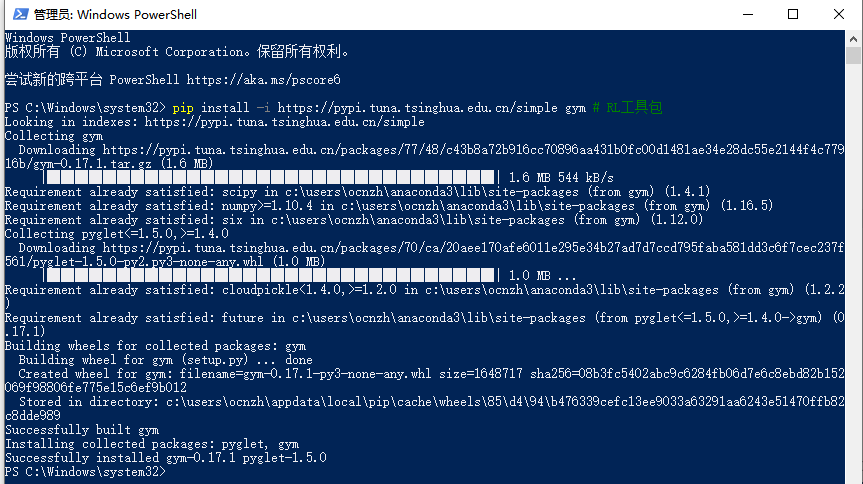
\includegraphics[width=0.6\textwidth]{Gyminstall.PNG}
\caption{gym 工具包}
\label{Gyminstall}
\end{figure}

%%%%%%%----------------------------------------
(\textbf{Q学习算法原理}\cite{Yutao2011})\index{Q学习算法}\index{Reinforcement Learning}
Q学习是 Watkins 提出, 并由 Watkins 与 Dayan 于 1992 年基本证明其收敛性 \cite{watkins1992q}.
Q学习利用状态–动作对值函数 $Q(s,a)$ 进行迭代, 其最优策略使得期望折扣报酬总和最大.
Q学习的值函数定义如下:
\begin{eqnarray}
  Q(s,a) =R(s,s^{'}, a) + \gamma\sum_{s^{'}\in S}P(s,s^{'}, a)\max_{a\in A}A(s^{'},a)
\end{eqnarray}
式 中 $\gamma(0 <\gamma< 1)$ 为折扣因子, 本文的 $\gamma$ 值取 0.9;
$P(s|s^{'},a)$ 为状态 $s$ 在控制动作 $a$ 发生后转移到状态 $s^{'}$ 的概率; agent会根据当前状态 $s$ 选择某一动作 $a$, 得
到下一状态 $s^{'}$ 及报酬值 $R(s,s^{'},a)$, 然后根据其报酬值及下式迭代寻优最大 $Q$ 值:
\begin{eqnarray}
  \left\{\begin{array}{ll}
    &Q^{k+1}(s_k,a_k)=Q^{k}(s_k,a_k)+\alpha[R(s_k,s_{k+1},a_k)+\gamma\max\limits_{a^{'}\in A}Q^{k}(s_{k+1},a_k)-Q^{k}(s_k,a_k)]\\
    &Q^{k+1}(\tilde{s},\tilde{a})=Q^{k}(\tilde{s},\tilde{a}),\forall (\tilde{s},\tilde{a})\neq (s_k,a_k).
  \end{array}\right.
\end{eqnarray}
式中: $Q^k$ 代表最优值函数 $Q^{*}$ 的第 $k$ 次迭代值; $\alpha(0 <\alpha< 1)$是学习因子, 它控制动作更新速度, $\alpha$ 值越小,算法的搜索空间越大, 算法的稳定性越好, 本文 $\alpha$ 值取 0.1.
Q学习算法在当前状态下总是选择具有最高 Q 值的动作, 称为贪婪策略 $\pi^{*}$, 如下式:
\begin{eqnarray}
  \pi^{*}=\mathop{\arg\max}_{a\in A}Q^k (s,a).
\end{eqnarray}
Q算法的动作策略选择较为关键, 合适的动作策略能提高学习的收敛速度及收敛效果. 文中采用一种基于概率分布选择动作的追踪算法
\cite{sutton1998reinforcement} 来构造动作选择策略. 在该策略下, 初始状态各动作被选择的概率相等, 但随着动作值函数的不断迭代, 越高的Q值的动作被选择的概率越大, 故Q算法最终将收敛于Q矩阵代表的最优策略.
该策略概率迭代公式如下:
\begin{eqnarray}
  \left\{\begin{array}{ll}
    &P^{k+1}_s(a)=P^k_s(a_g)+\beta(1-P^k_s(a_g));\\
    &P^{k+1}_s(a)=P^k_s(a)(1-\beta),\forall a\in A, a\neq a_g;\\
    &P^{k+1}_{\tilde{s}}(a)=P^k_{\tilde{s}}(a),\forall a\in A, \forall \tilde{s}\in S,\tilde{s}\neq s.\\
  \end{array}\right..
\end{eqnarray}
在每一状态下, 对应于 Q 最大值的动作称为贪婪动作, 记为 $a_g$. 式中 $\beta(0 <\beta < 1)$ 值的大小决定了动作搜索的速度, $\beta$ 值越接近1说明控制动作策略越趋于贪婪策略, 本文 $\beta$ 值取 0.5.
$P^k_s(a)$ 代表第 $k$ 次迭代时状态 $s$ 下选择动作 $a$ 的概率.
在经过足够迭代次数的探索和利用之后, $Q^k$ 将会以概率1收敛于最优值函数 $Q^{*}$, 最终得到一个 $Q^{*}$ 矩阵表示的最优控制策略.

%%%%%%%----------------------------------------
\index{Q-Learning Algorithm Used for Average Reward}
\textbf{平均奖励Q-Learning算法} (\textbf{Q-Learning algorithm used for average reward}) \cite{gosavi2004reinforcement}.

\textbf{步骤 1}. 令所有$Q(l,u) \leftarrow 0$. $k=$是状态变化数. $\rho^k=0$表示第$k$阶段平均奖赏估计. $W=0$, 程序最大运行次数$k_{\max}$, $k_{\max}$应足够大. 从任意状态喀什系统的仿真. 选取一个特殊状态$s^{*}$.

\textbf{步骤 2}. 当前状态记为$i$. 以概率$1/|A (i)|$选取动作, 其中$A(i)$ 记状态$i$允许的所有动作集. 状态$i$的贪婪动作状态$i$得最高Q-值关联.

\textbf{步骤 3}. 仿真动作$a$. 下一状态记为$j$. 令$r(i, a, j)$为在动作$a$下, 从$i$到$j$的奖赏. 更新律$Q(i,a)$定义为
\begin{eqnarray}
  Q(i,a)\leftarrow (1-\alpha(k))Q(i,a)+\alpha(k)[r(i,a,j)-\rho^k+M_b^j],
\end{eqnarray}
其中$M_b^j= 0$ if $j = s$ (称为\textbf{SSP grounding})\index{SSP Grounding}, 否则 $M^j_b= \max_{b\in A}(j)Q(j,b)$.

\textbf{Step 4}. 对于步骤2选出的贪婪动作, 按如下方式更新$W$: $W \leftarrow W + r(i, a, j)$, $\rho^k$按如下方式更新:
\begin{eqnarray}
  \rho^{k+1}= (1 - \beta(k))\rho^k+ \beta(k)\frac{W}{k}.
\end{eqnarray}

\textbf{Step 5}. 若$k < k_{\max}$, 令$i \leftarrow j, k \leftarrow k + 1$, 返回步骤2. 否则转步骤6.

\textbf{Step 6}. 对于状态$i$, 选取$\mu(i)\in  \mathop{\arg\max}_{a\in A }(i)Q(i, a)$. 解策略$\mu$由算法得到 , 算法停止.

%\textbf{Q-Learning Algorithm} \cite{Rahimiyan2010-5452971,Weissensteiner2009-5061503}, \cite{AraabiBN2007-4126273, AdamS2012-5719642}, \cite{MoodyJ2001-935097,
%Kao-ShingHwang2004-1321086} \index{Q-Learning Algorithm}
%%%%%%%---------------------------------------------
\section{作业}

%%%%%%---------------------------------
\begin{think}
 什么是三段论推理?
\end{think}

%%%%%%---------------------------------
\begin{think}
  什么是自然演绎推理?
\end{think}

%%%%%%---------------------------------
\begin{think}
判断下列表达式对是否可以合一?如果可以合一,给出最一般合一 (MGU)

1) $P(x,b,b), P(a, y, z)$;

2) $P(x,f(x)),P(y,y)$;

3) $2+3=x,x=3+3$.
\end{think}

%%%%%%---------------------------------
\begin{think}
  对所有的x、y、z来说, 如果y是x父亲, z是y的父亲,则z是x的道每个, 又知每个人都有父亲, 试问是否会有这样的个人X和Y, 使得X是Y的祖父?
\end{think}
